\documentclass[t,darkblue]{beamer}
\usepackage[portuguese]{babel}
\usepackage[utf8]{inputenc}
\usepackage{times}
\usepackage[T1]{fontenc}
\usepackage{hyperref}
\usepackage[alf]{abntex2cite}
\usepackage{tikz}
\usepackage{listings}
\usepackage{xcolor}
\usepackage[export]{adjustbox}
\usepackage{lipsum}
\usepackage{caption}			% Pacote para retirar o prefixo "Figura"
\captionsetup[figure]{labelformat=empty}% redefines the caption setup of the figures environment in the beamer class.
\usepackage{parskip}
\setlength{\parskip}{\baselineskip} 

\renewcommand{\raggedright}{\leftskip=0pt \rightskip=0pt plus 0cm}
\newcommand\fontvi{\fontsize{9}{9}\selectfont}

% Definição de estilo

\usetheme{Madrid} 
%\setbeamertemplate{background}{\tikz[overlay,remember picture]\node[opacity=0.4]at (current page.center){\includegraphics[width=2cm]{Imagens/Logomarca}};} % Marca d'água por trás do texto

% Definição de fonte
\usefonttheme[onlylarge]{structurebold}
\setbeamerfont*{frametitle}{size=\normalsize,series=\bfseries}

% Definição de cores
\definecolor{icmcAzulLogo}{RGB}{121,178,242}
\definecolor{icmcAzulSite}{RGB}{66,135,214}
\definecolor{icmcAzulBorda}{RGB}{66,135,214}

% Range de cores do template
\setbeamercolor{structure}{fg=icmcAzulBorda!90!icmcAzulSite}

% Declaração alternativa da palheta de cores do modelo
%\mode<presentation>
%{
%	\usetheme{Madrid}
%	\setbeamercolor*{palette primary}{use=structure,fg=white,bg=icmcAzulSite}
%	\setbeamercolor*{palette secondary}{use=structure,fg=white,bg=icmcAzulLogo}
%	\setbeamercolor*{palette tertiary}{use=structure,fg=white,bg=icmcAzulBorda}
%}

\begin{document}
	\author[Aula 04]{Dados rasters e compositor de impressão}
	\title[Dados rasters, compositor de impressão]{Como dominar o mundo com geoprocessamento}
	\subtitle{Aula 04}
	\titlegraphic{\vspace{-1cm}
\includegraphics[width=2.0cm]{./image/vale}\hspace*{6.75cm}~%
		
\includegraphics[width=1.5cm]{./image/qgis}\\
		
\includegraphics[width=2.5cm]{./image/tetra}}
	\institute[]{Alexandre Assunção}
	\date{20 de maio de 2025}
	%\subject{}
	%\setbeamercovered{transparent}
	\setbeamertemplate{navigation symbols}{}
	\begin{frame}[plain]
	\maketitle
	\end{frame}

% Conteúdo
\begin{frame}
\frametitle{Sumário da Aula 04}
\large
\begin{itemize}
	\item Importação e união de dados alfanuméricos; e
	\item Geração de curvas de nível e mapa hipsométrico;
	\item Compositor de impressão (layout);
\end{itemize}
\end{frame}

\begin{frame}
	\frametitle{Geração de curvas de nível e mapa hipsométrico}
	\begin{figure}[H]
		\centering
		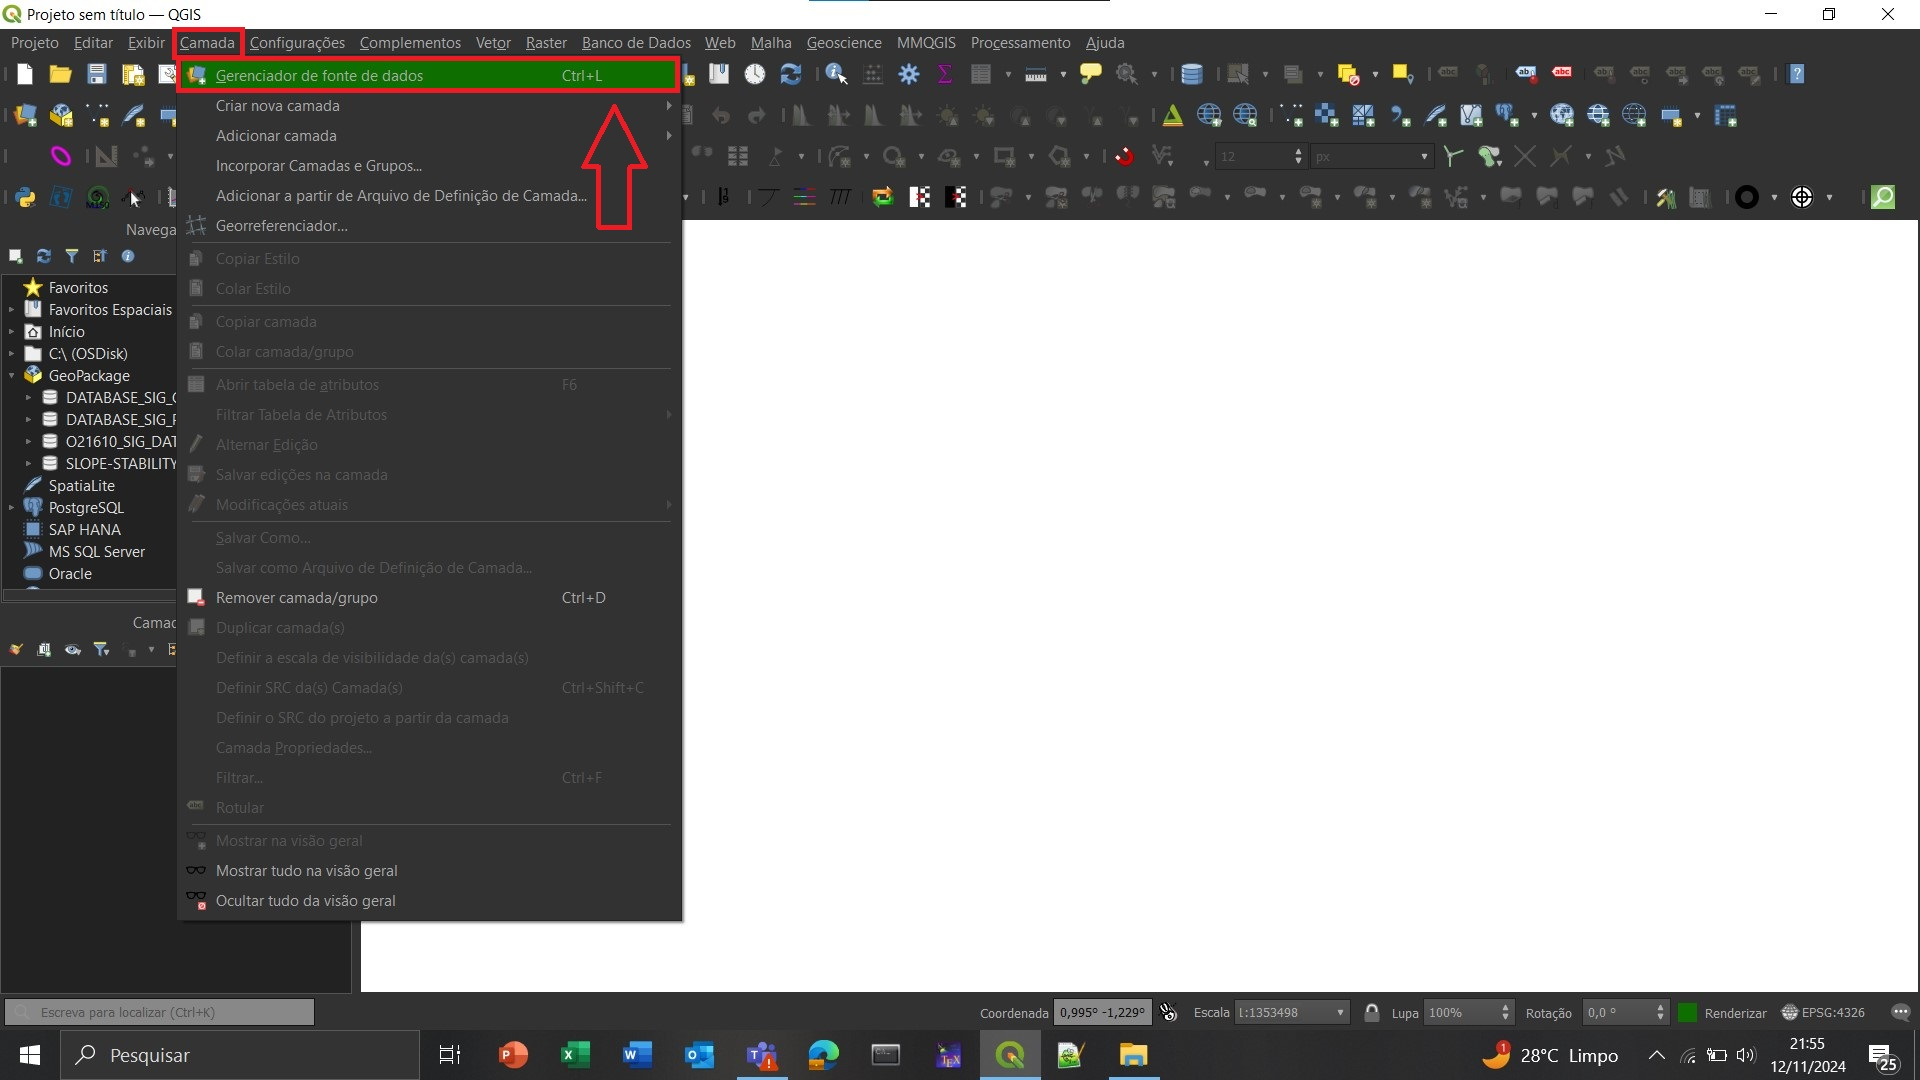
\includegraphics[width=\textwidth]{./image/hipso_1}
	\end{figure}
\end{frame}

\begin{frame}
	\frametitle{Geração de curvas de nível e mapa hipsométrico}
	\begin{figure}[H]
		\centering
		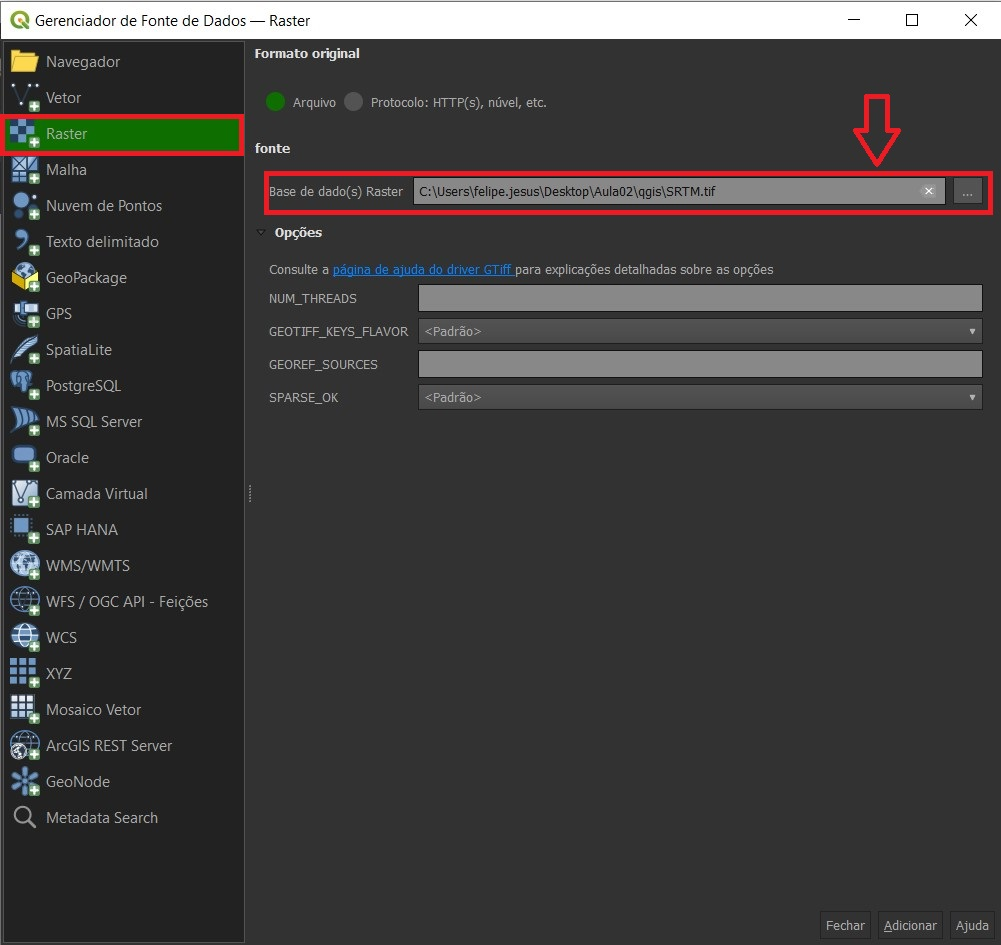
\includegraphics[width=0.7\textwidth]{./image/hipso_2}
	\end{figure}
\end{frame}

\begin{frame}
	\frametitle{Geração de curvas de nível e mapa hipsométrico}
	\begin{figure}[H]
		\centering
		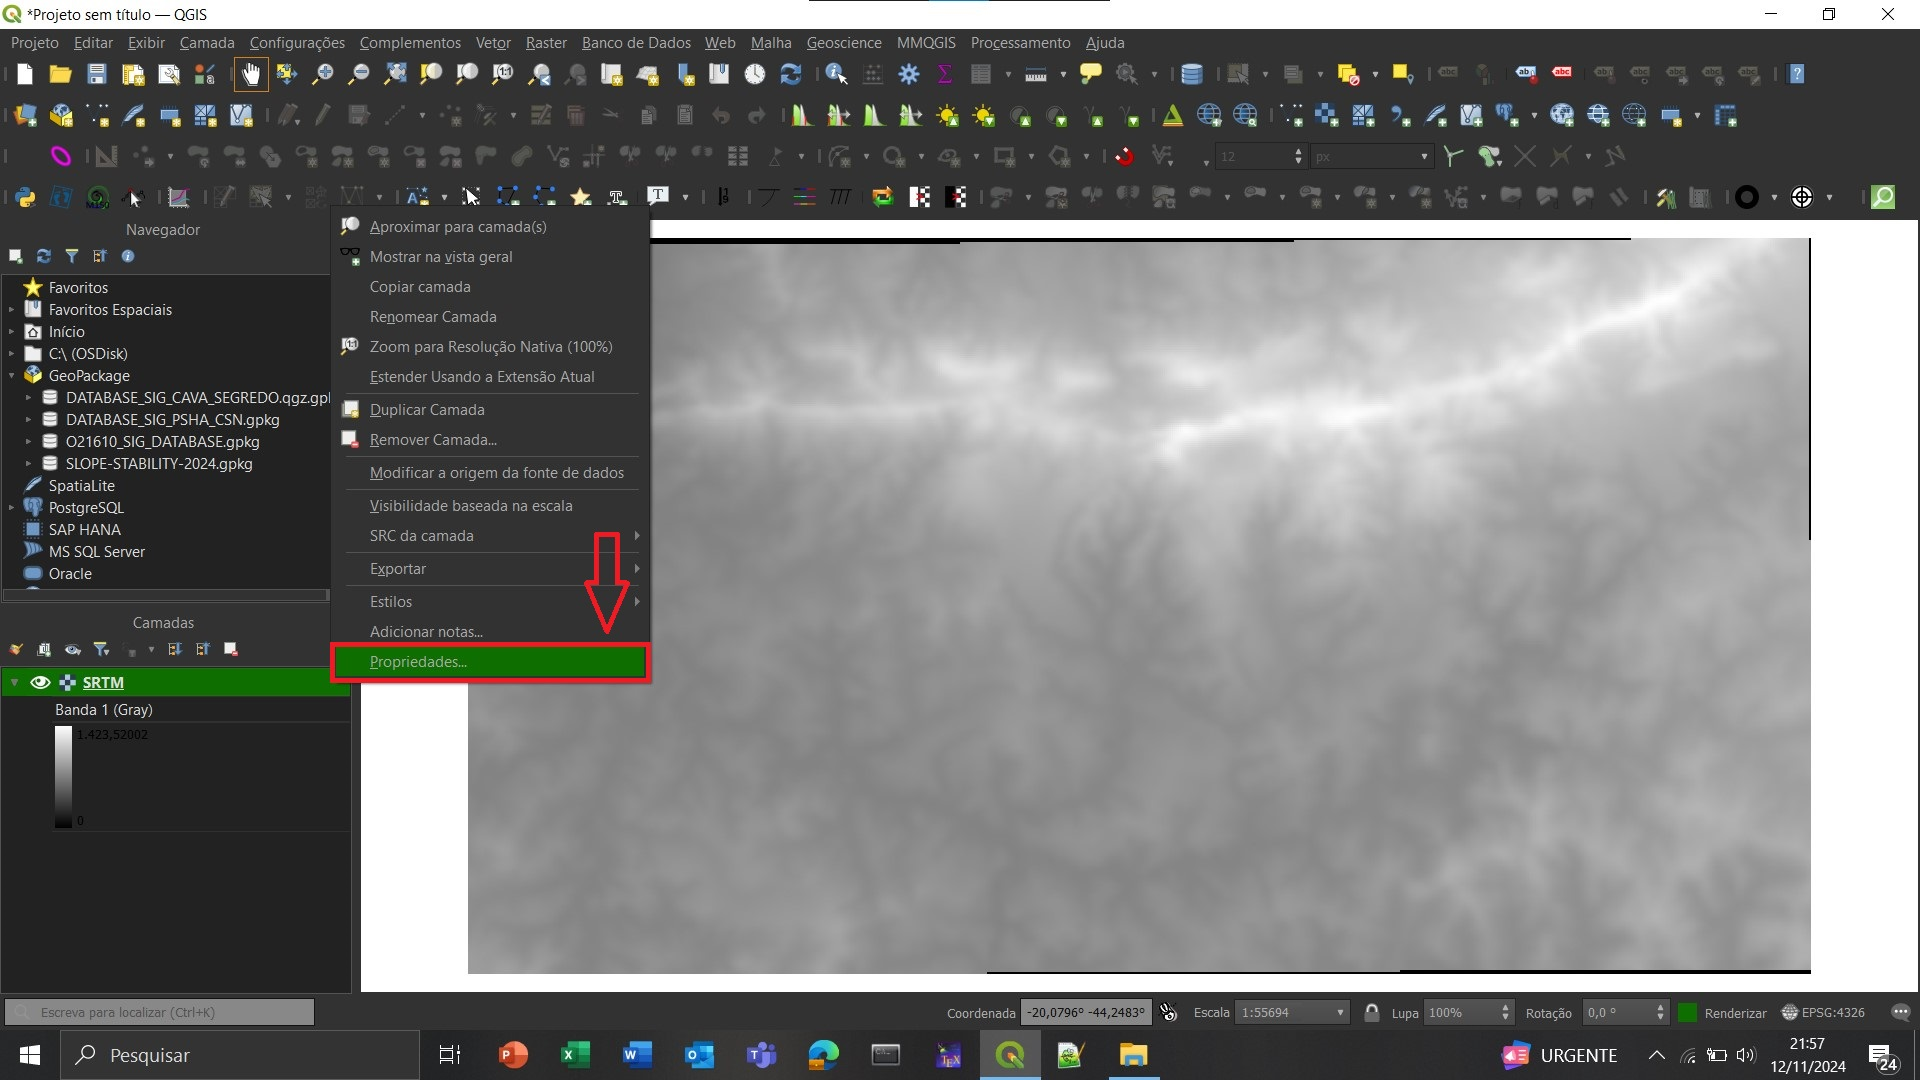
\includegraphics[width=\textwidth]{./image/hipso_3}
	\end{figure}
\end{frame}

\begin{frame}
	\frametitle{Geração de curvas de nível e mapa hipsométrico}
	\begin{figure}[H]
		\centering
		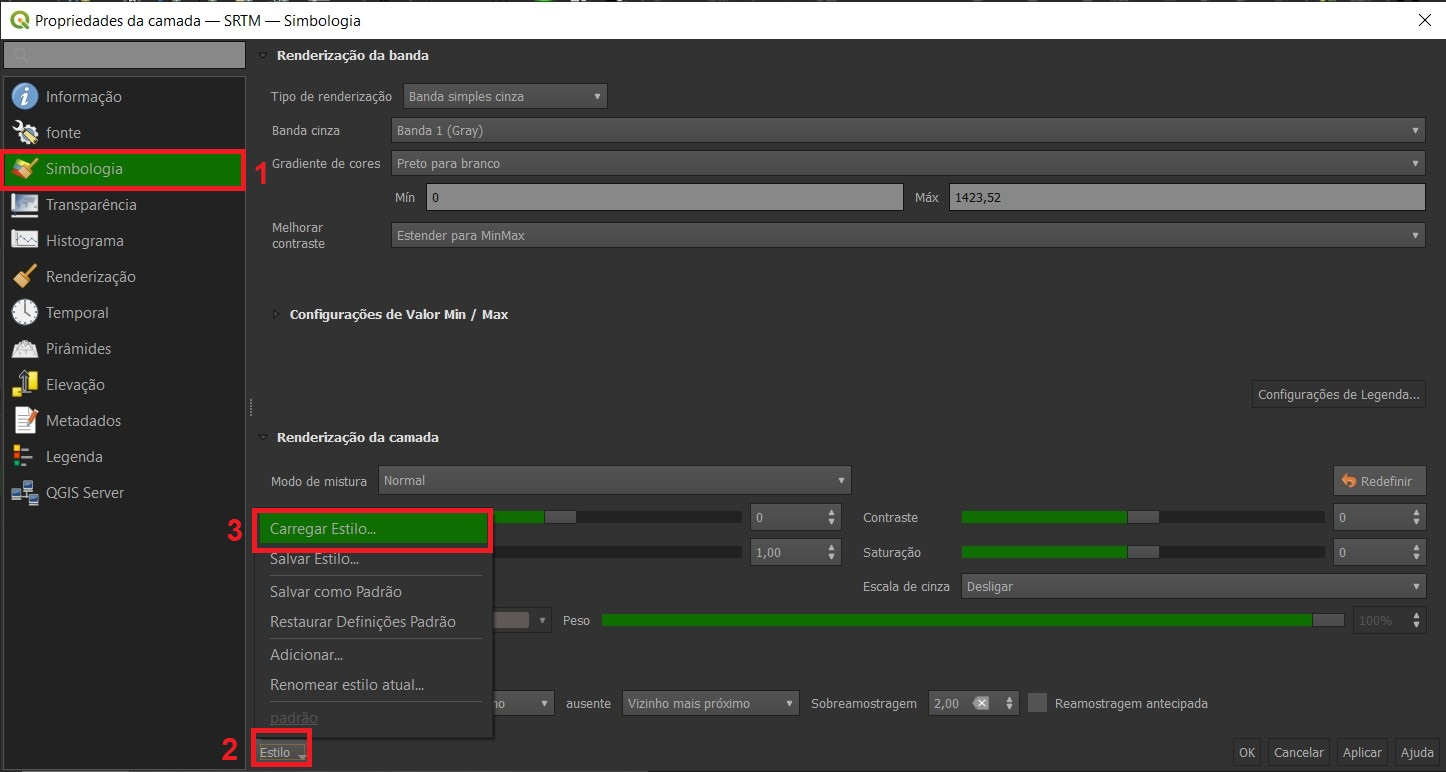
\includegraphics[width=\textwidth]{./image/hipso_4}
	\end{figure}
\end{frame}

\begin{frame}
	\frametitle{Geração de curvas de nível e mapa hipsométrico}
	\begin{figure}[H]
		\centering
		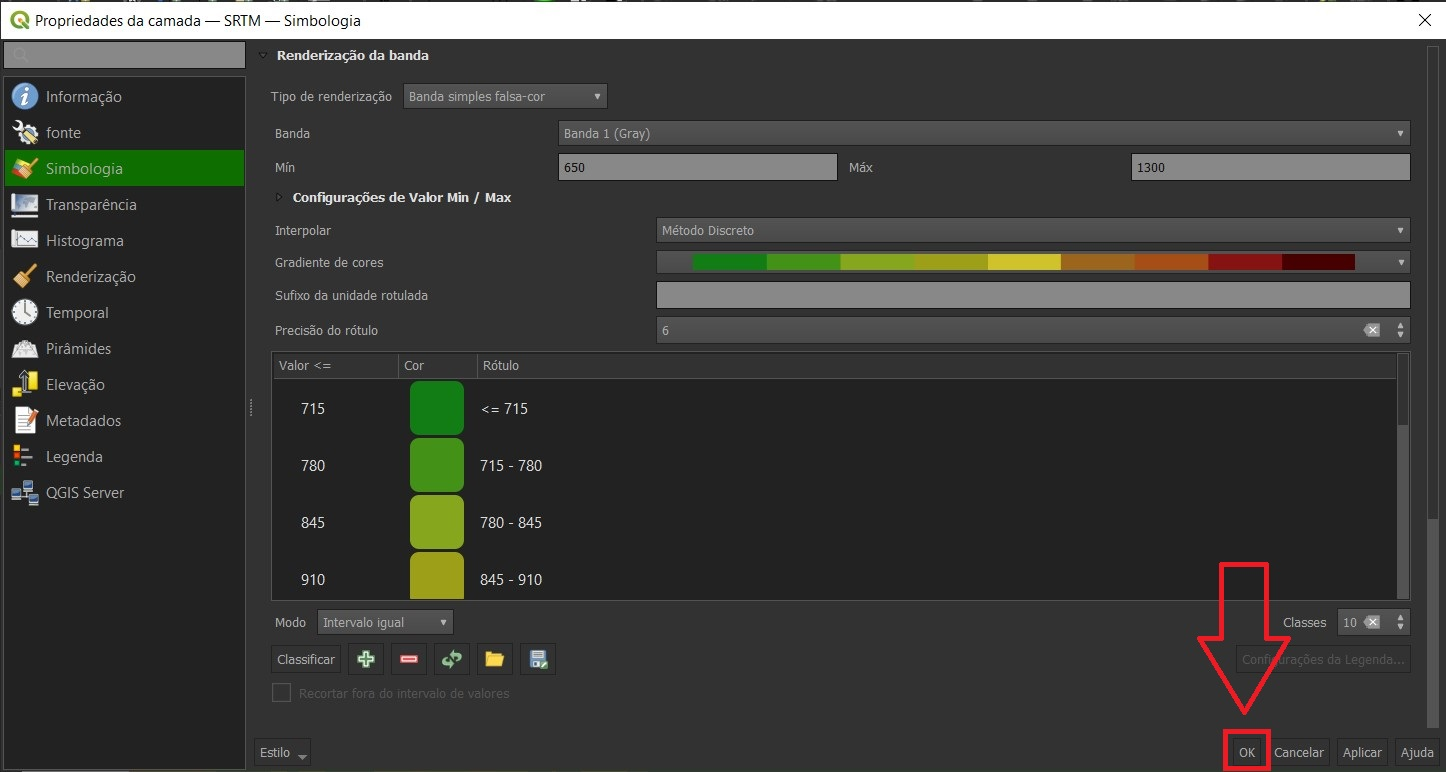
\includegraphics[width=\textwidth]{./image/hipso_5}
	\end{figure}
\end{frame}

\begin{frame}
	\frametitle{Geração de curvas de nível e mapa hipsométrico}
	\begin{figure}[H]
		\centering
		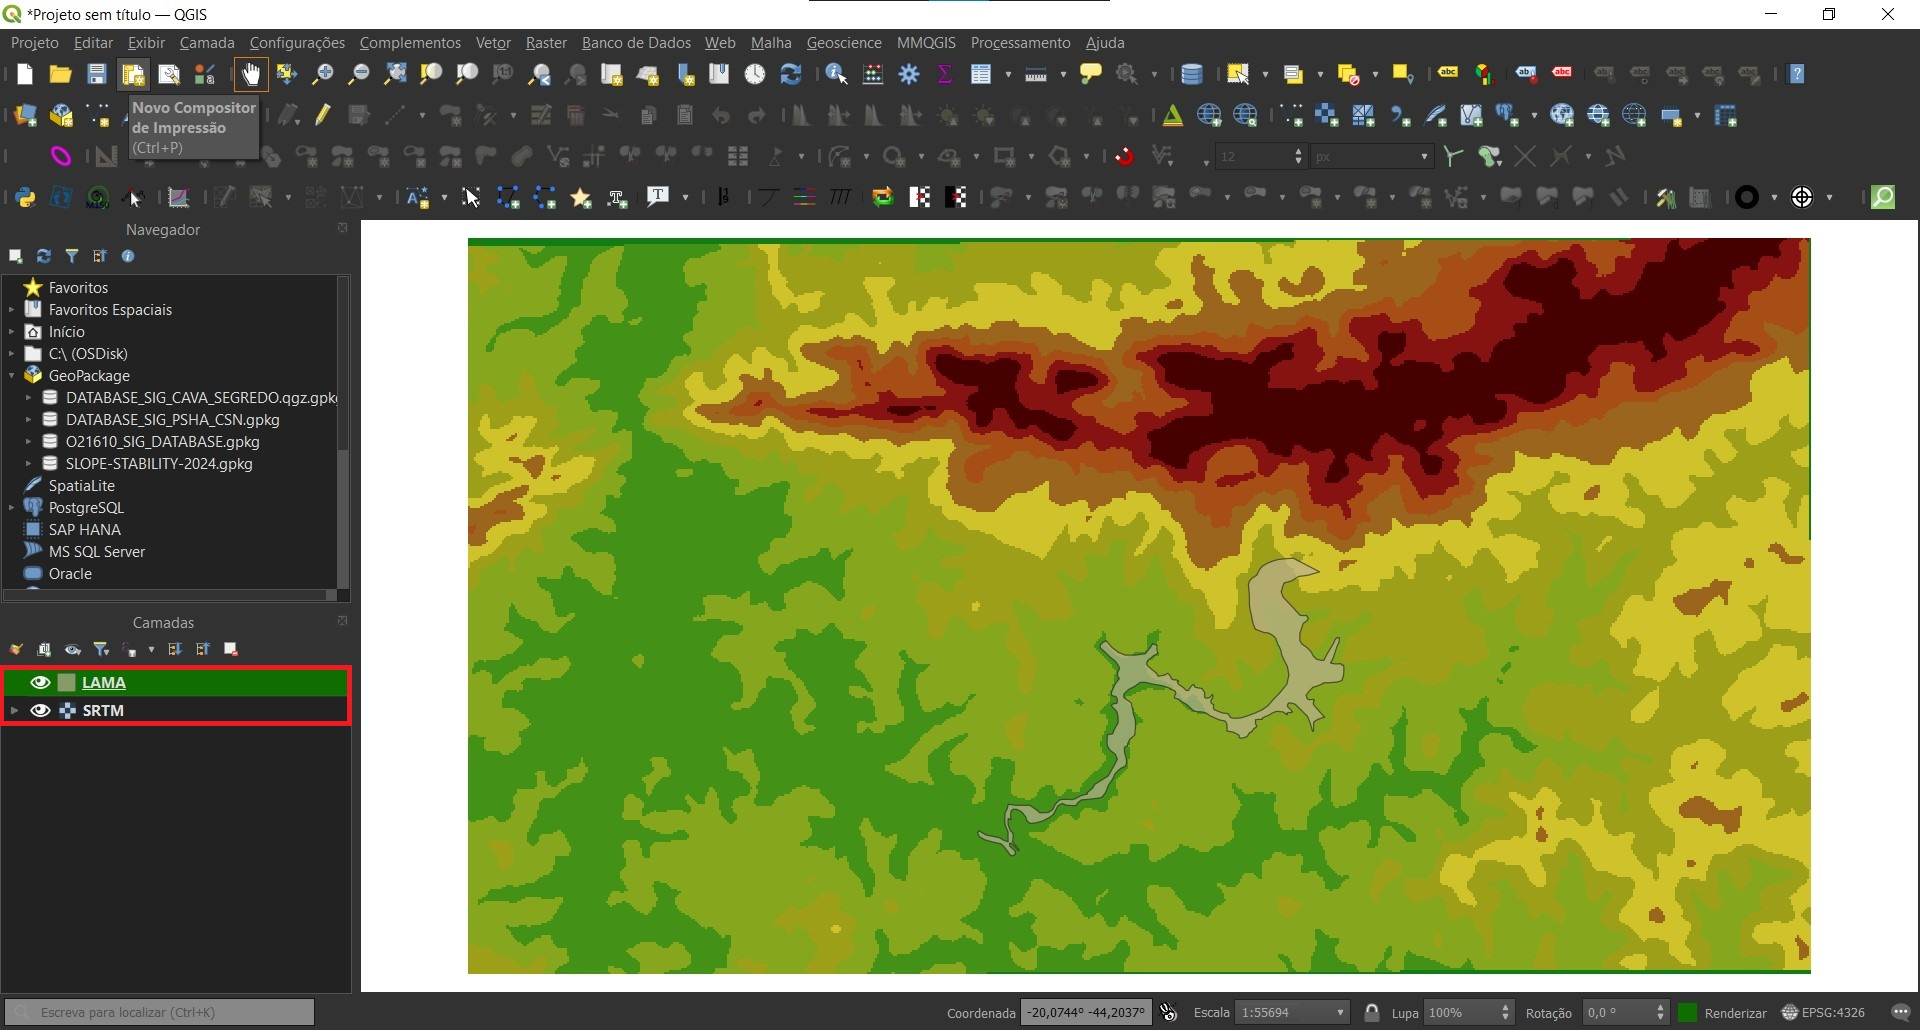
\includegraphics[width=\textwidth]{./image/hipso_8}
	\end{figure}
\end{frame}

\begin{frame}
	\frametitle{Geração de curvas de nível e mapa hipsométrico}
	\begin{figure}[H]
		\centering
		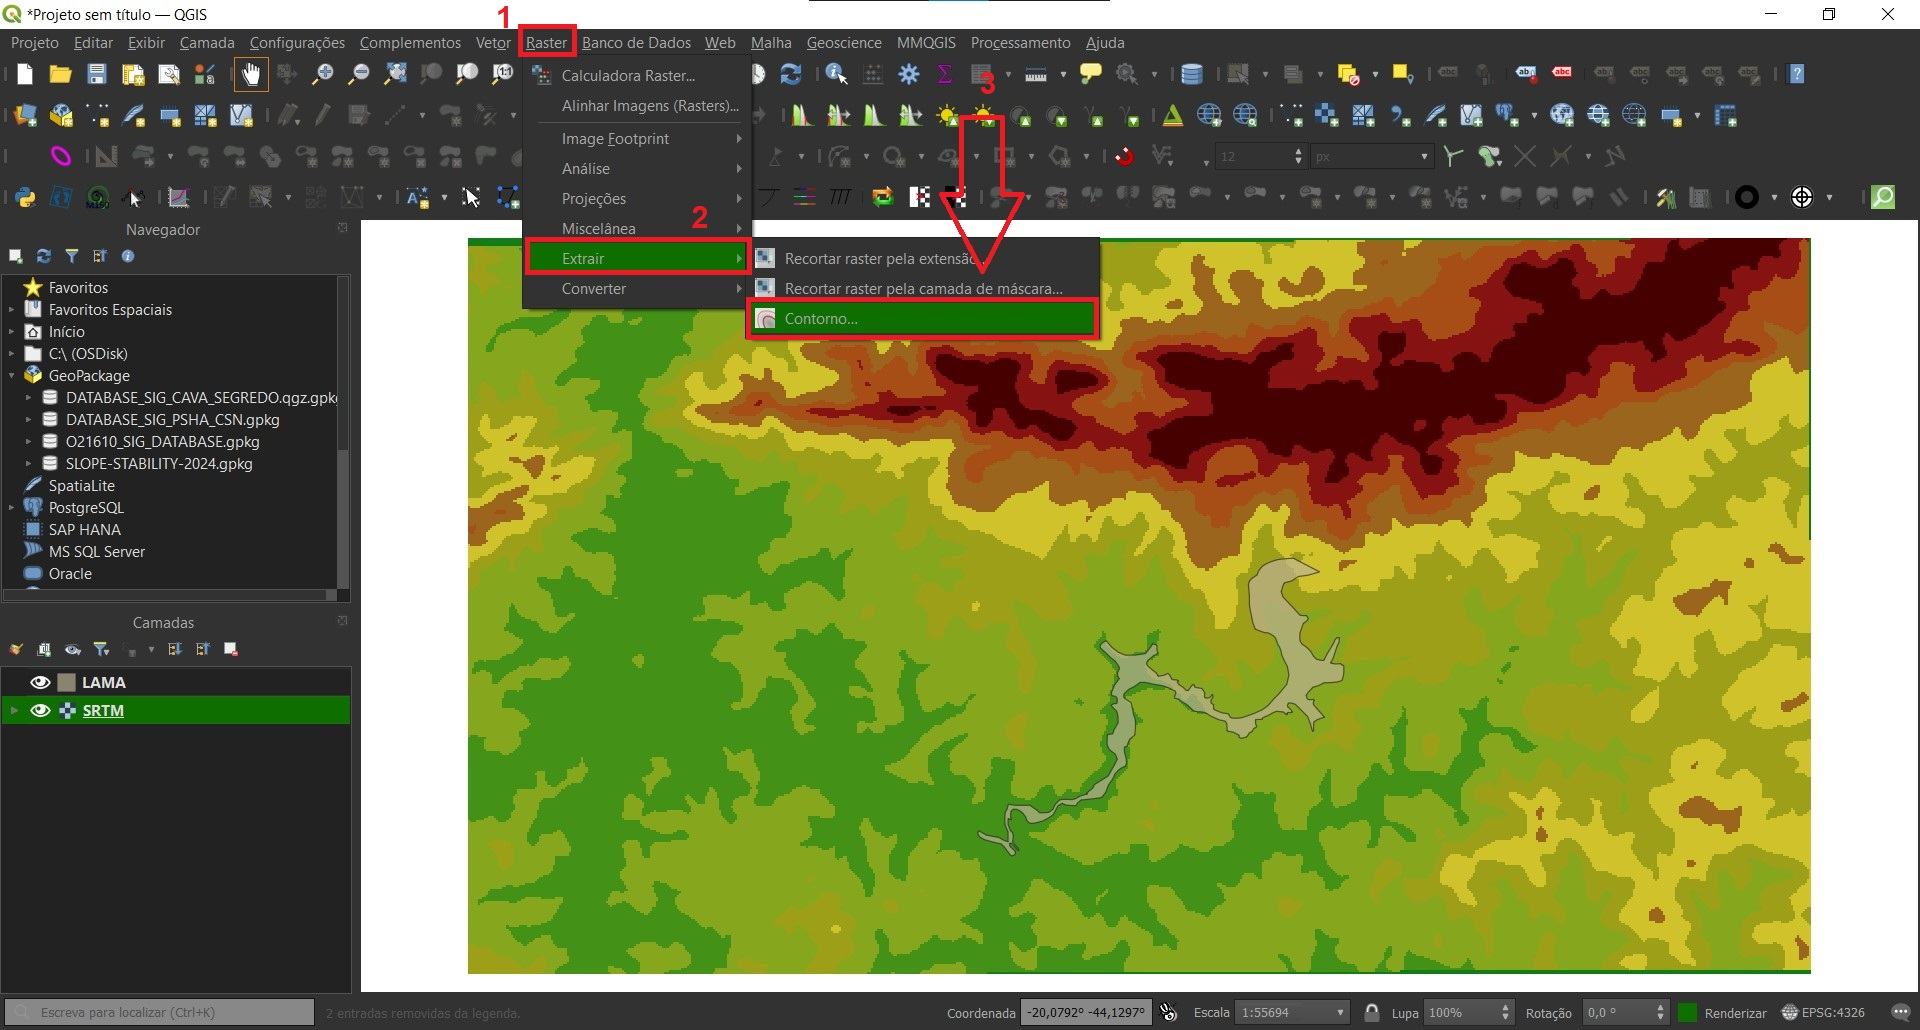
\includegraphics[width=\textwidth]{./image/hipso_9}
	\end{figure}
\end{frame}

\begin{frame}
	\frametitle{Geração de curvas de nível e mapa hipsométrico}
	\begin{figure}[H]
		\centering
		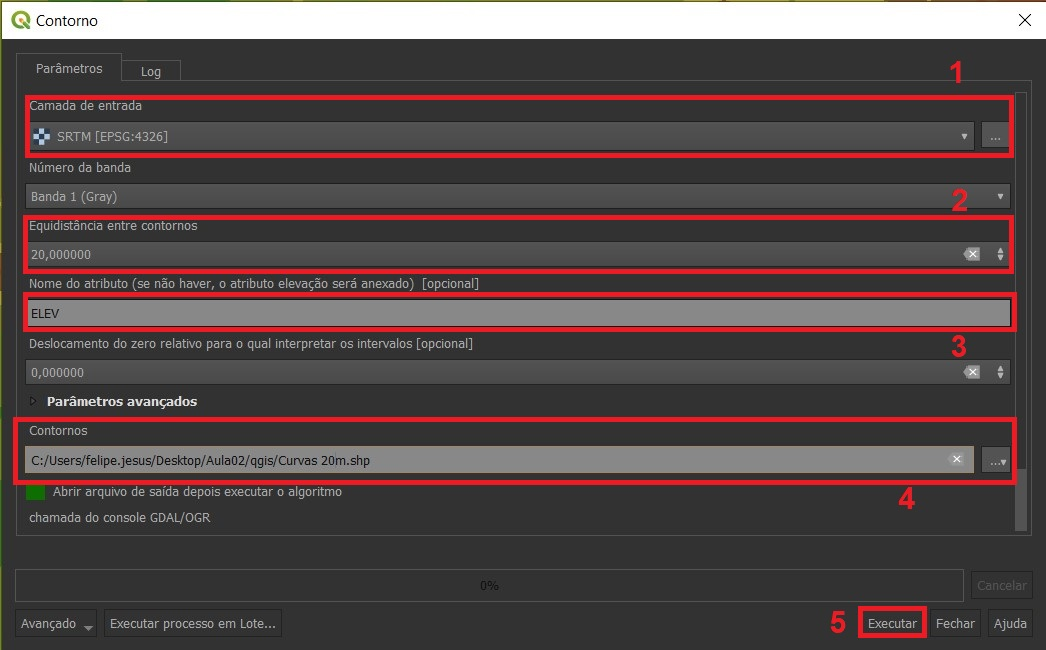
\includegraphics[width=\textwidth]{./image/hipso_10}
	\end{figure}
\end{frame}

\begin{frame}
	\frametitle{Geração de curvas de nível e mapa hipsométrico}
	\begin{figure}[H]
		\centering
		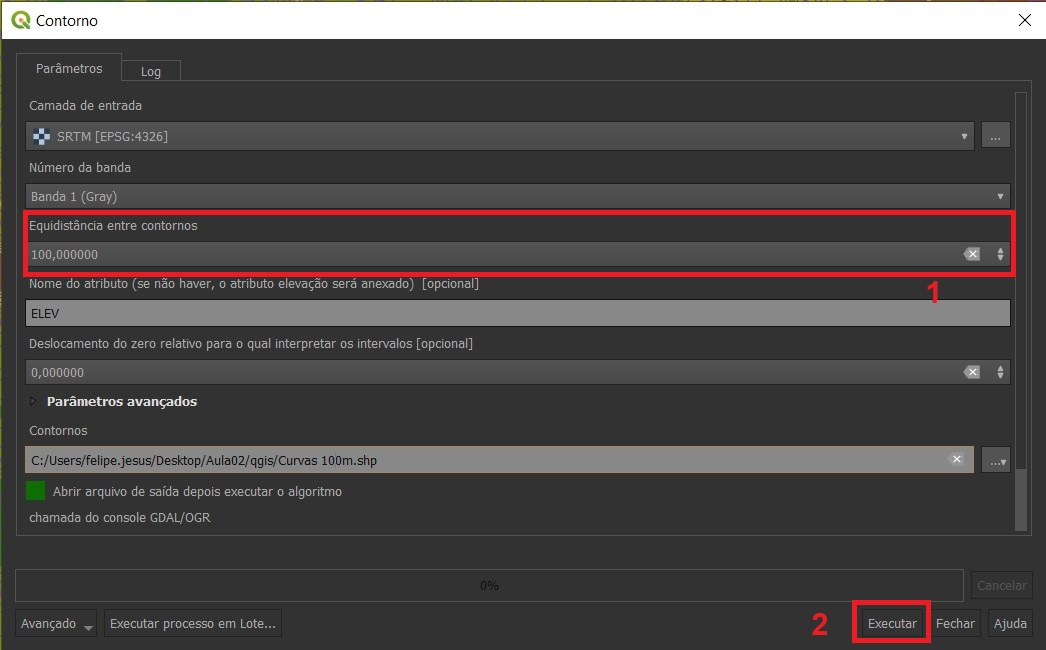
\includegraphics[width=\textwidth]{./image/hipso_11}
	\end{figure}
\end{frame}

\begin{frame}
	\frametitle{Geração de curvas de nível e mapa hipsométrico}
	\begin{figure}[H]
		\centering
		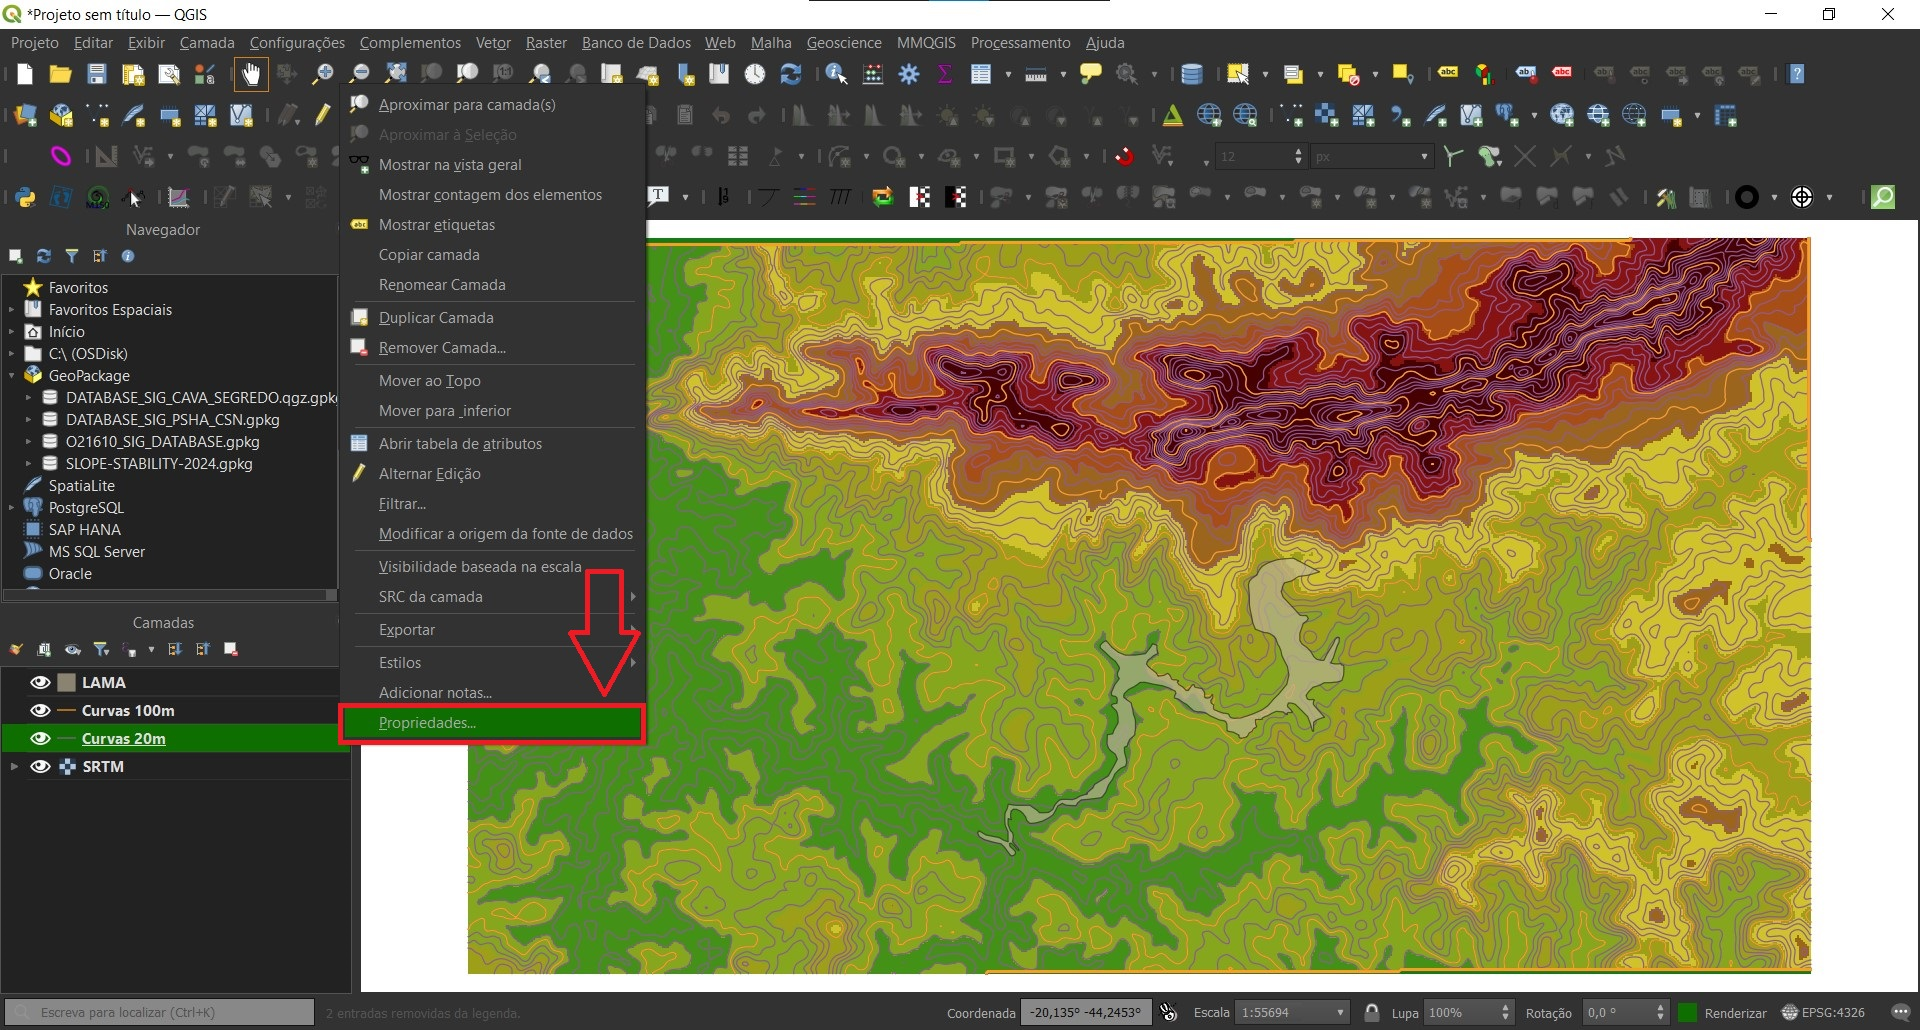
\includegraphics[width=\textwidth]{./image/hipso_12}
	\end{figure}
\end{frame}

\begin{frame}
	\frametitle{Geração de curvas de nível e mapa hipsométrico}
	\begin{figure}[H]
		\centering
		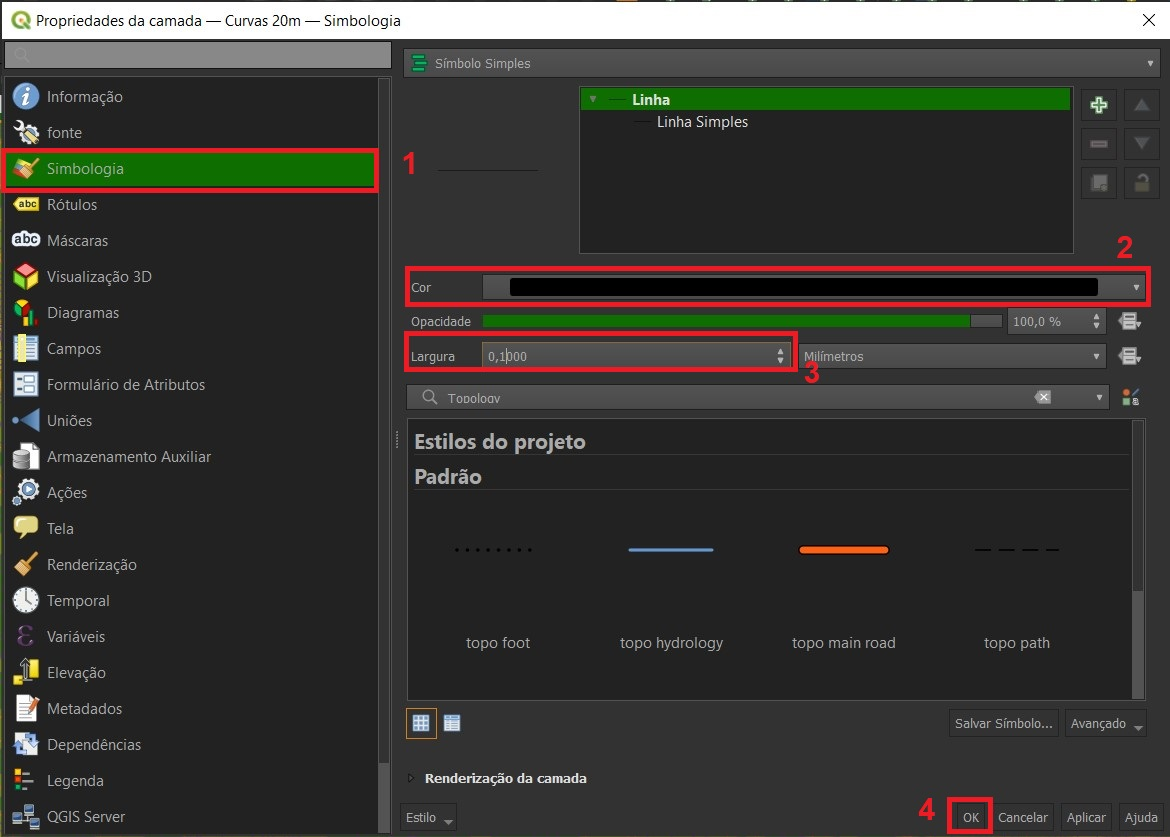
\includegraphics[width=0.85\textwidth]{./image/hipso_13}
	\end{figure}
\end{frame}

\begin{frame}
	\frametitle{Geração de curvas de nível e mapa hipsométrico}
	\begin{figure}[H]
		\centering
		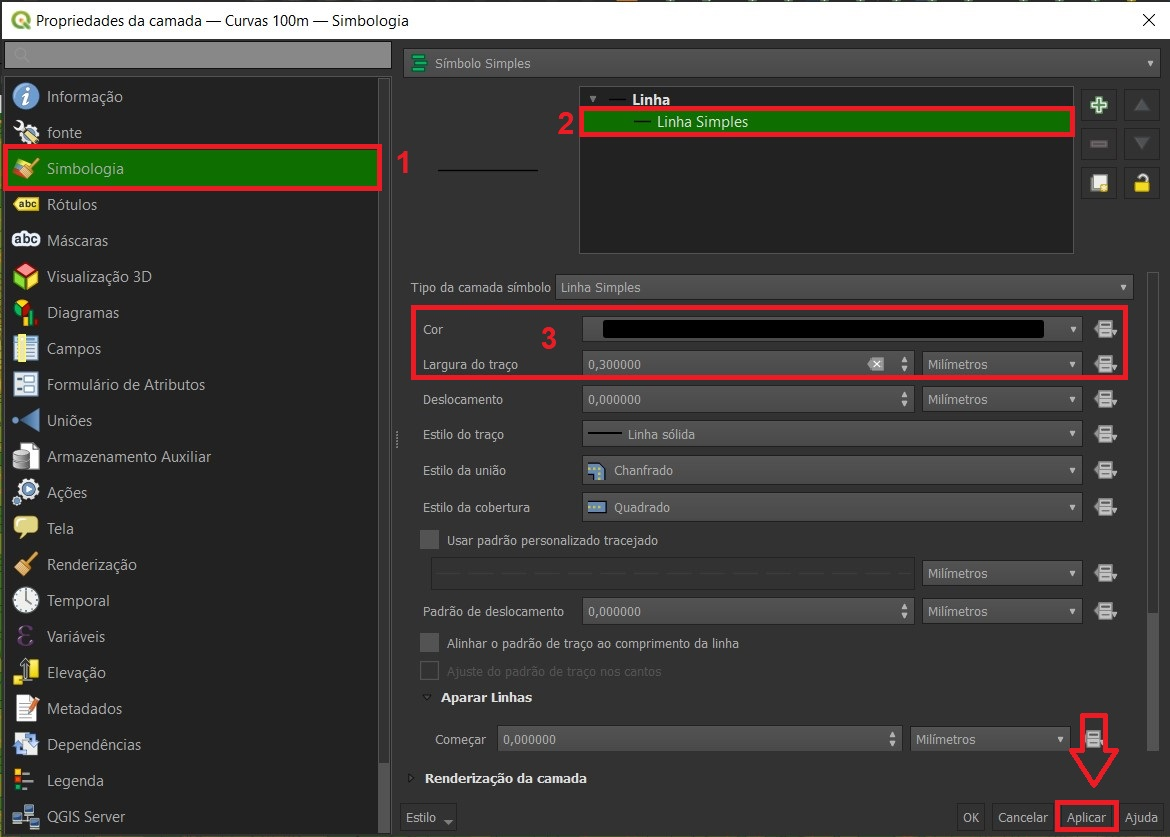
\includegraphics[width=0.85\textwidth]{./image/hipso_14}
	\end{figure}
\end{frame}

\begin{frame}
	\frametitle{Geração de curvas de nível e mapa hipsométrico}
	\begin{figure}[H]
		\centering
		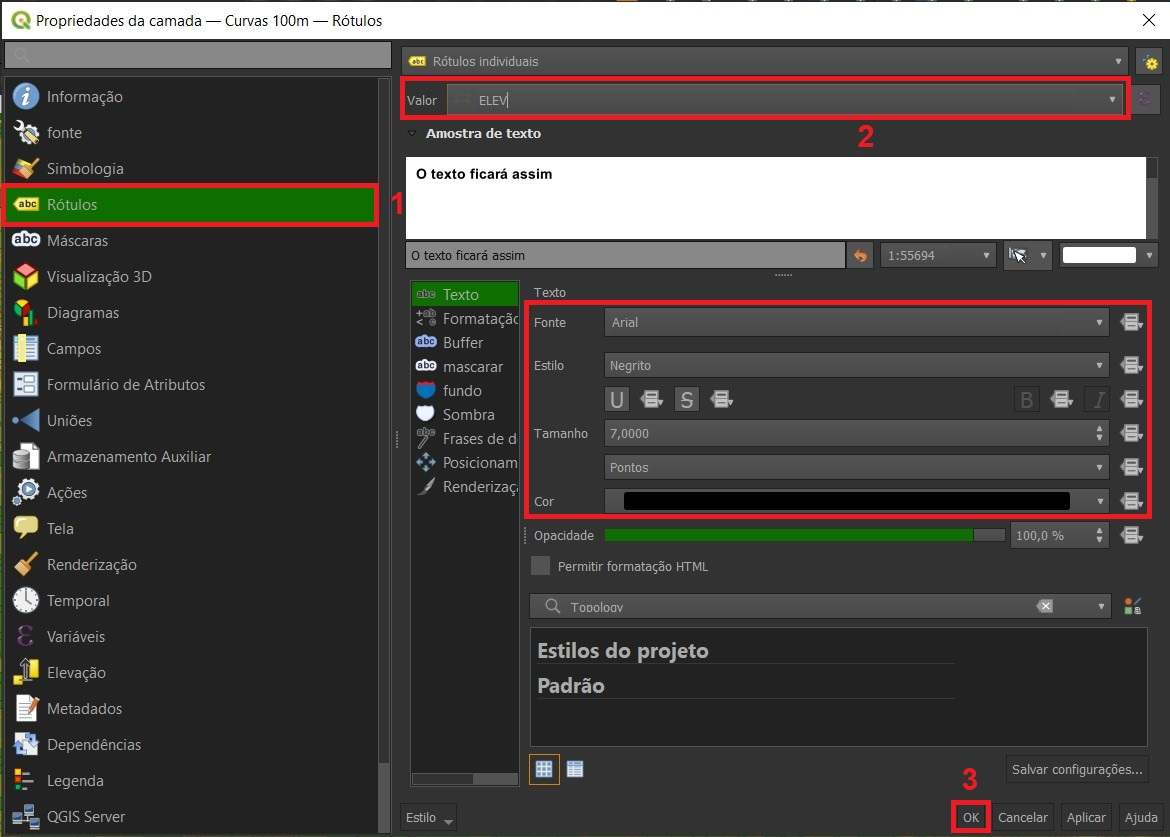
\includegraphics[width=0.85\textwidth]{./image/hipso_15}
	\end{figure}
\end{frame}

\begin{frame}
	\frametitle{Geração de curvas de nível e mapa hipsométrico}
	\begin{figure}[H]
		\centering
		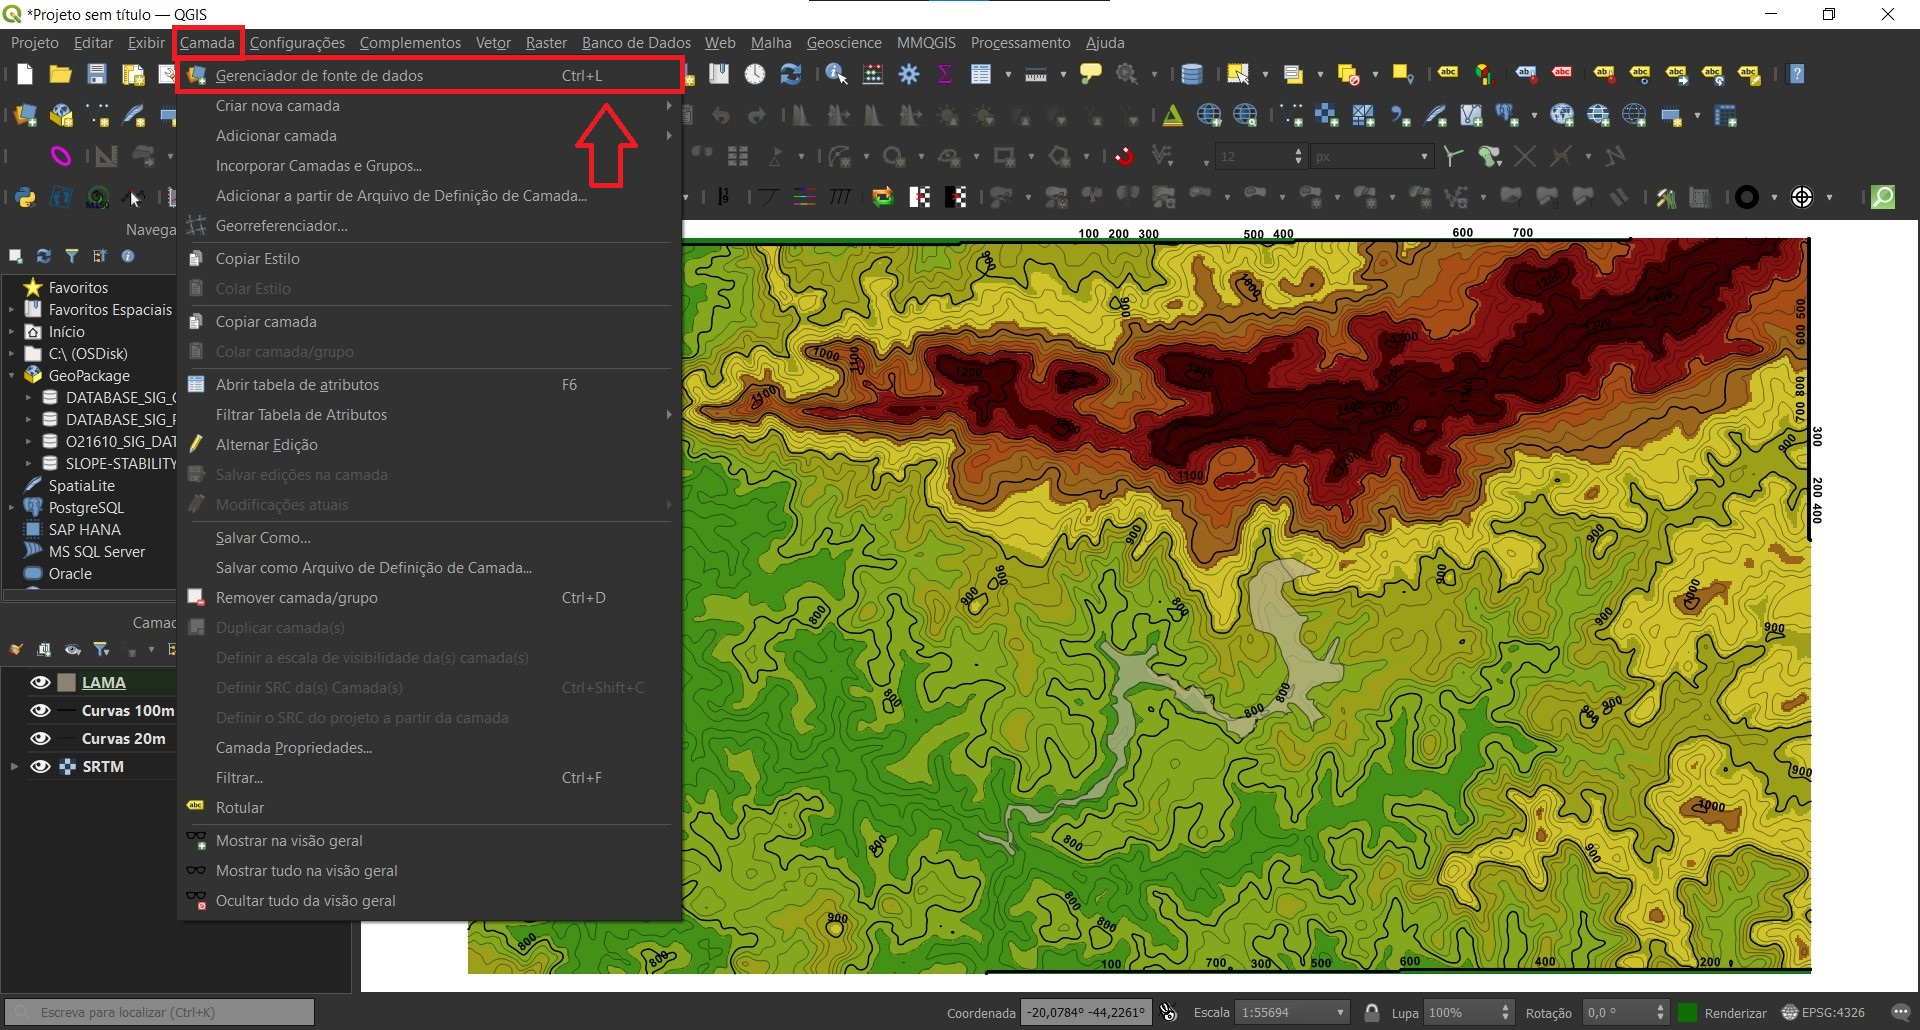
\includegraphics[width=\textwidth]{./image/hipso_16}
	\end{figure}
\end{frame}

\begin{frame}
	\frametitle{Geração de curvas de nível e mapa hipsométrico}
	\begin{figure}[H]
		\centering
		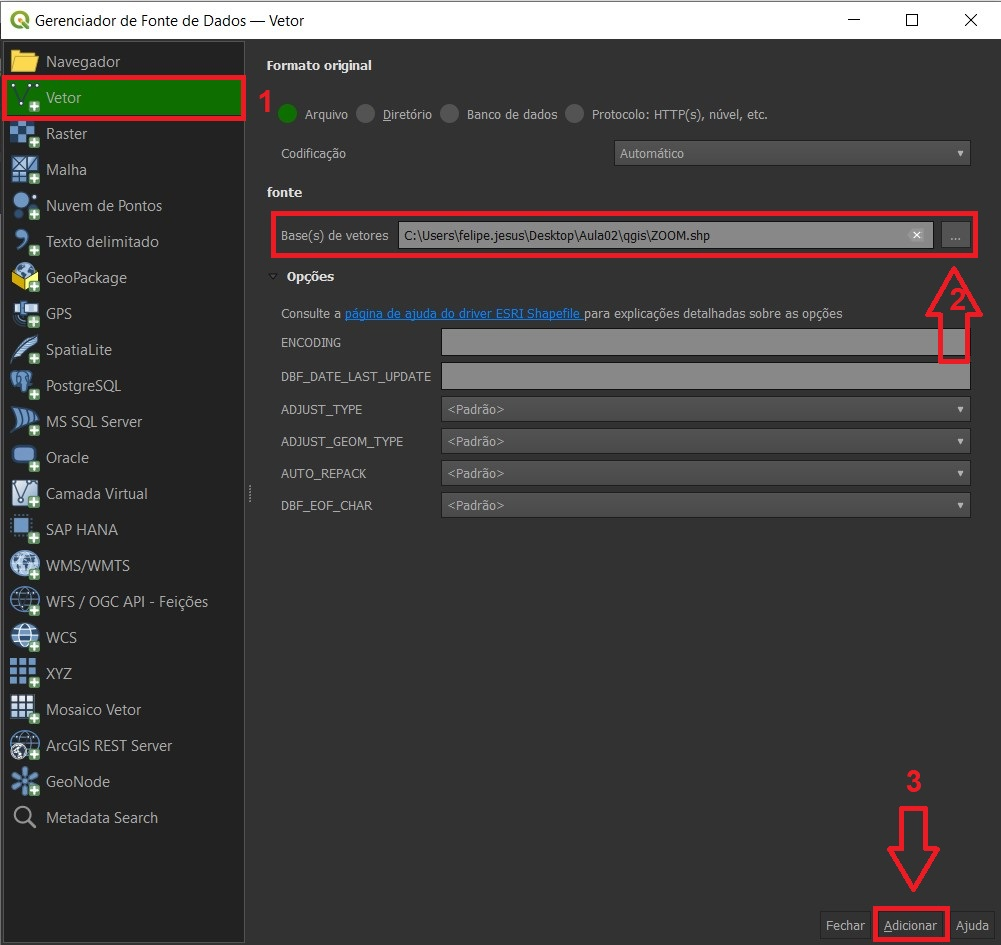
\includegraphics[width=0.7\textwidth]{./image/hipso_17}
	\end{figure}
\end{frame}

\begin{frame}
	\frametitle{Geração de curvas de nível e mapa hipsométrico}
	\begin{figure}[H]
		\centering
		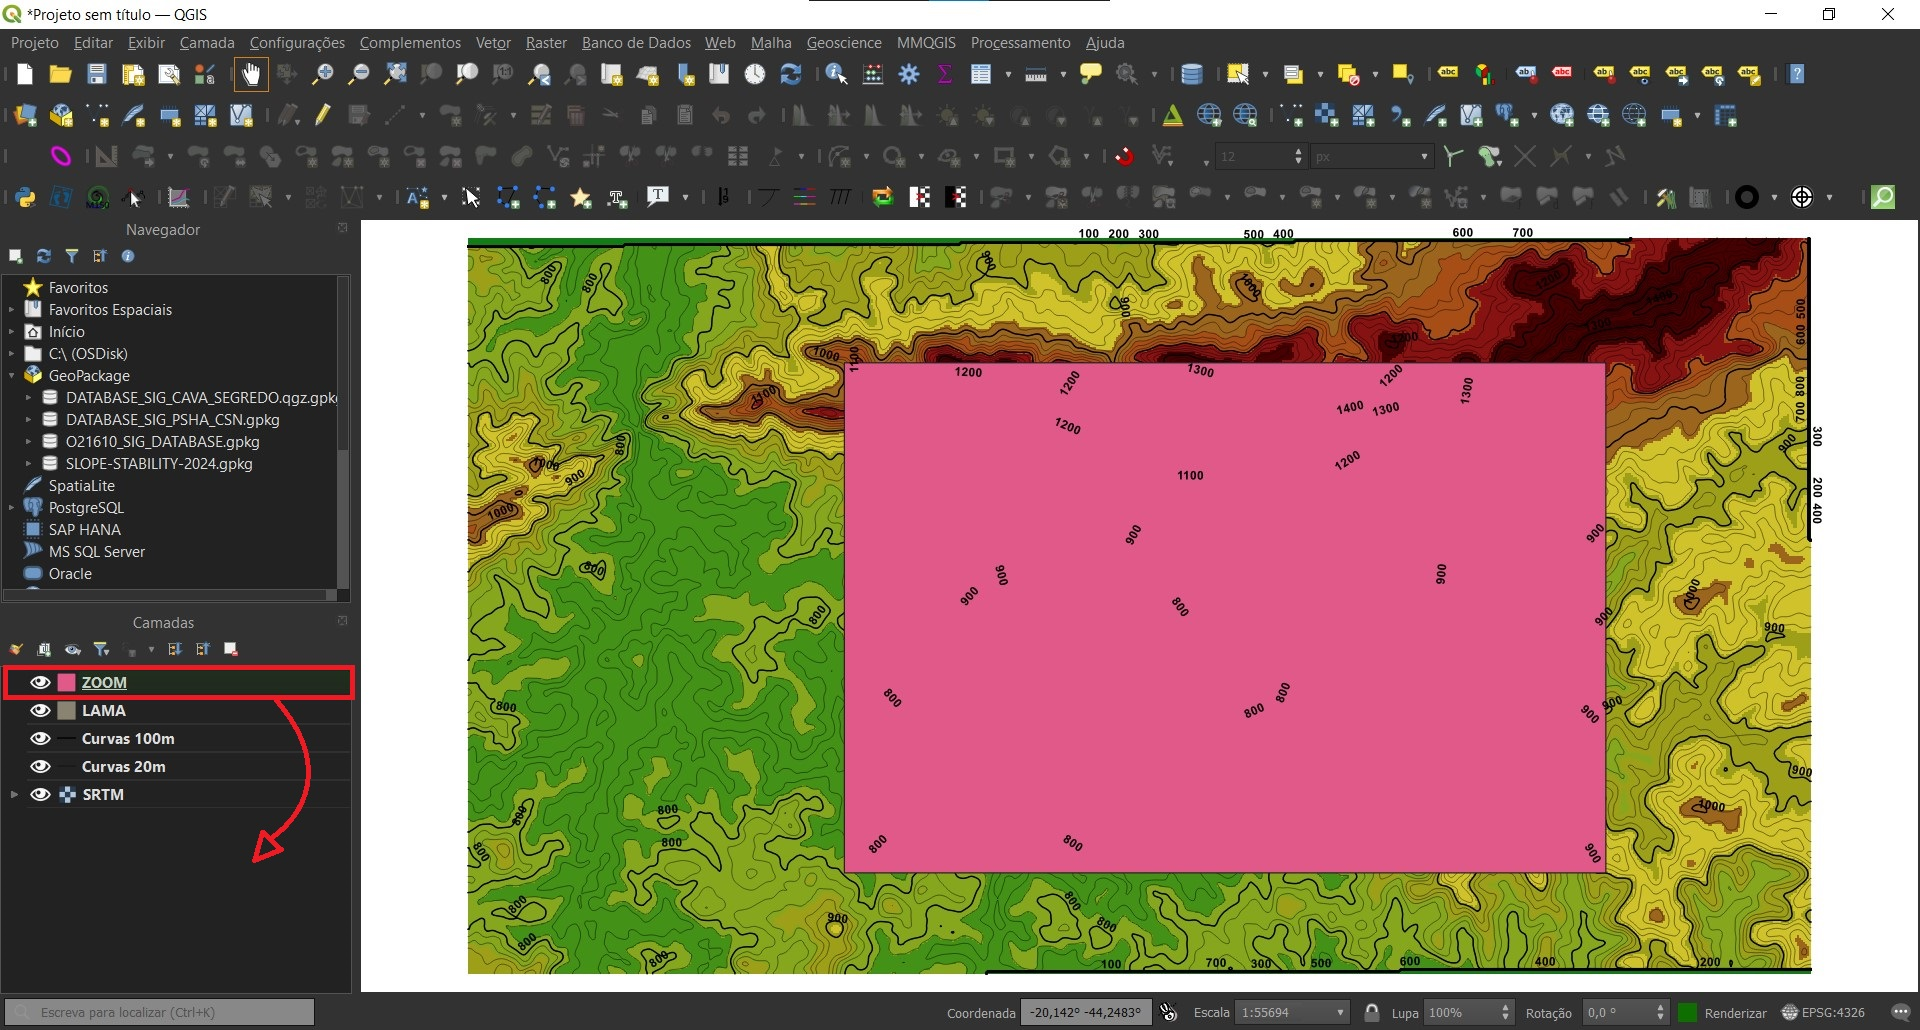
\includegraphics[width=\textwidth]{./image/hipso_18}
	\end{figure}
\end{frame}

\begin{frame}
	\frametitle{Geração de curvas de nível e mapa hipsométrico}
	\begin{figure}[H]
		\centering
		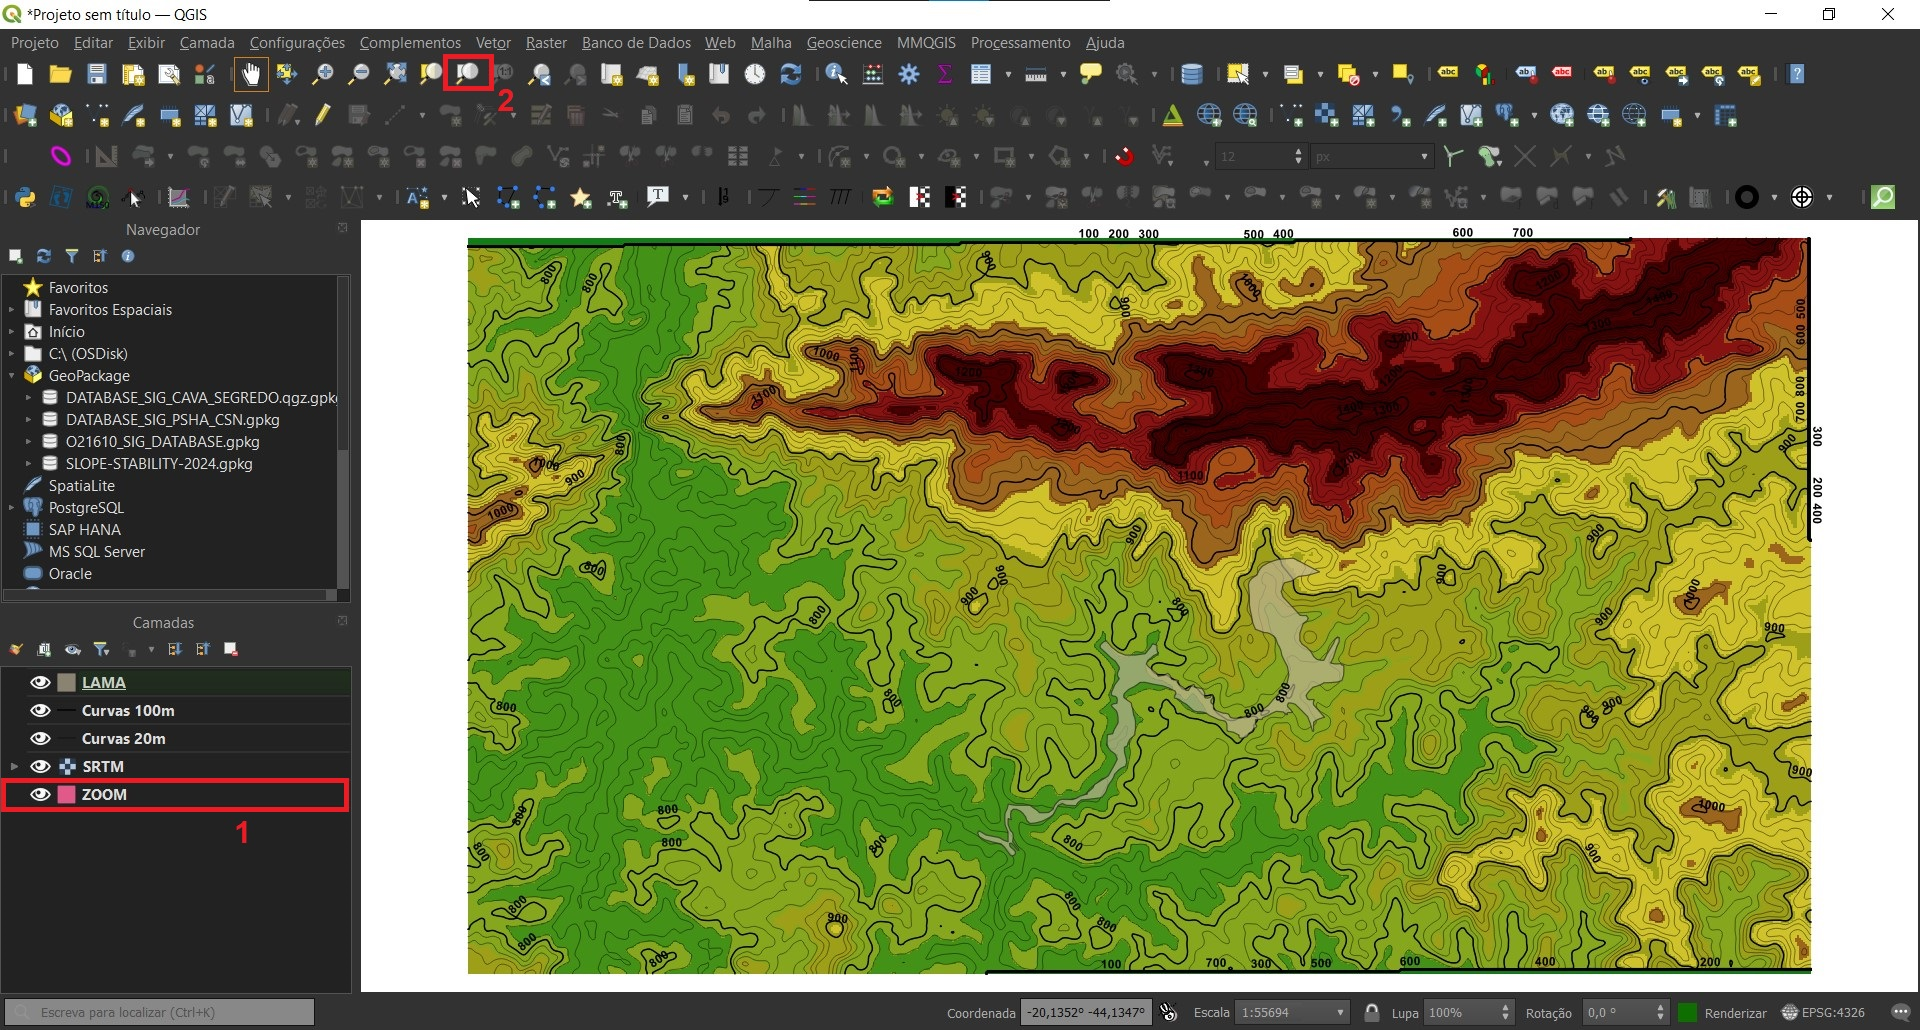
\includegraphics[width=\textwidth]{./image/hipso_19}
	\end{figure}
\end{frame}

\begin{frame}
	\frametitle{Geração de curvas de nível e mapa hipsométrico}
	\begin{figure}[H]
		\centering
		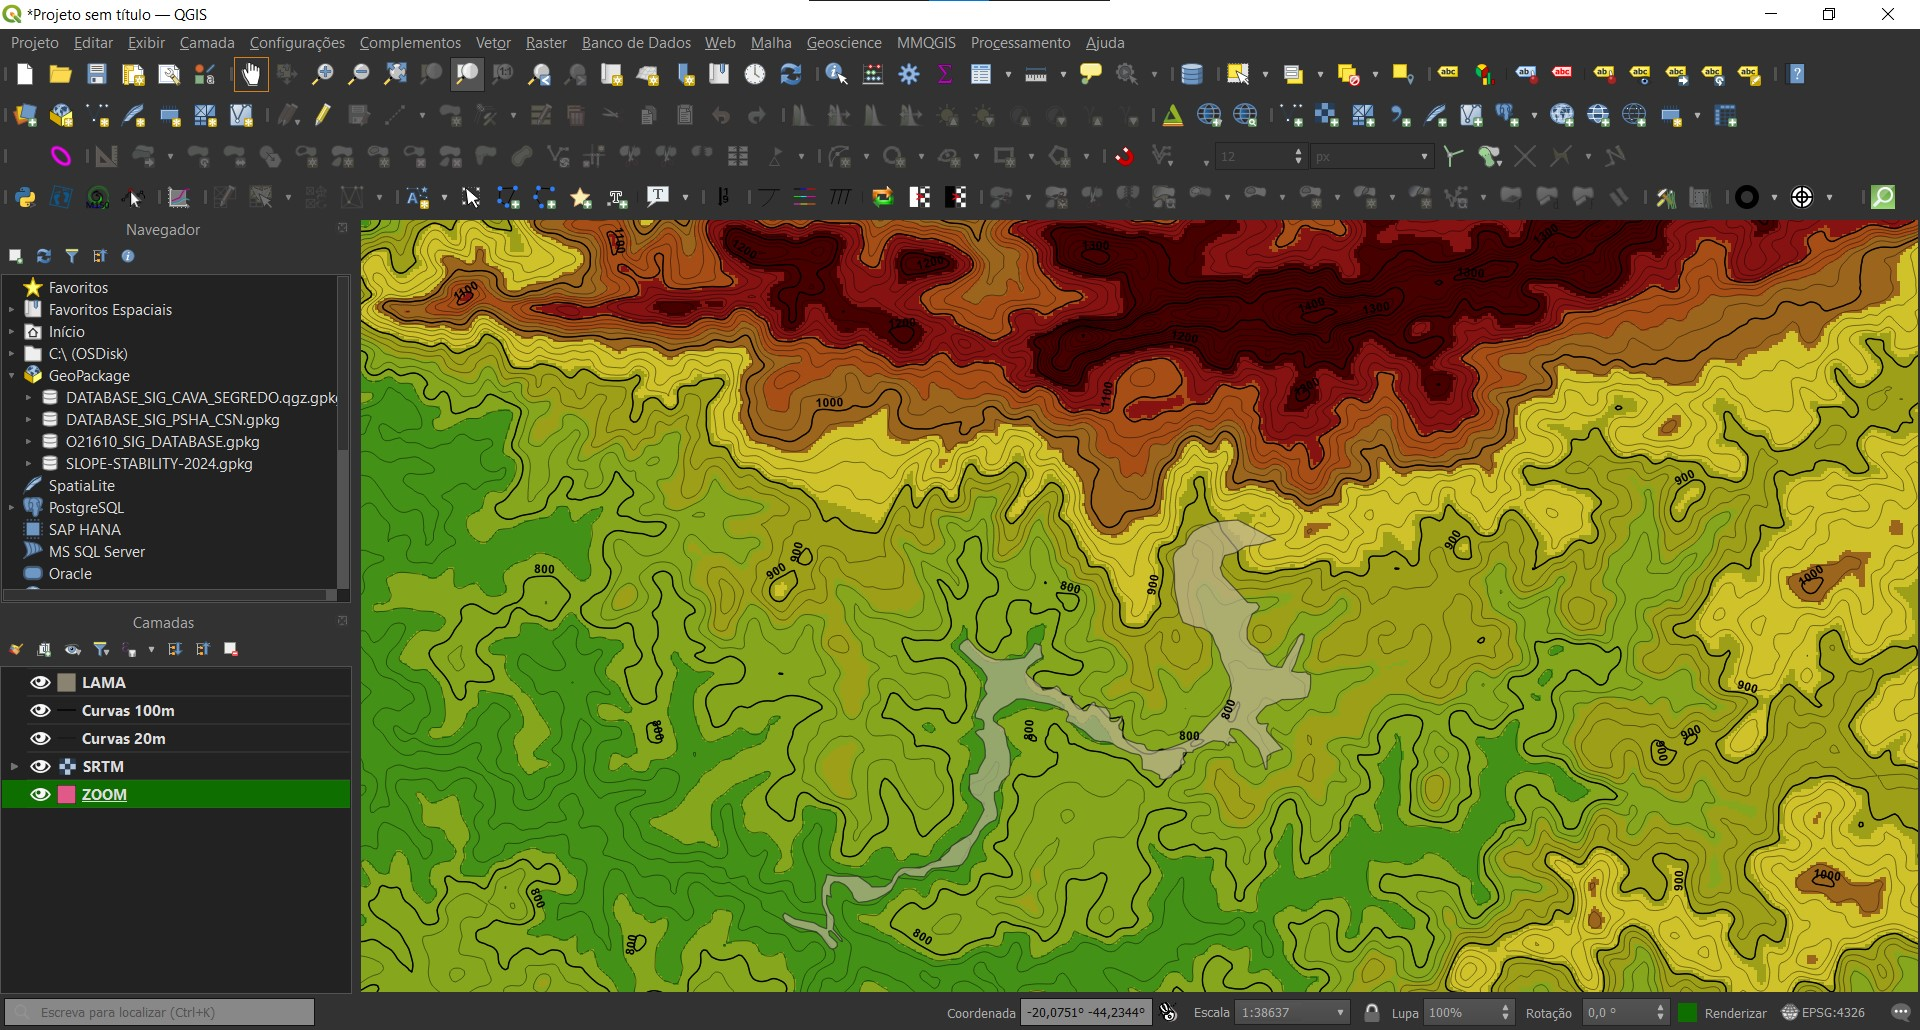
\includegraphics[width=\textwidth]{./image/hipso_20}
	\end{figure}
\end{frame}


\begin{frame}
	\frametitle{Compositor de impressão}
	\begin{figure}[H]
		\centering
		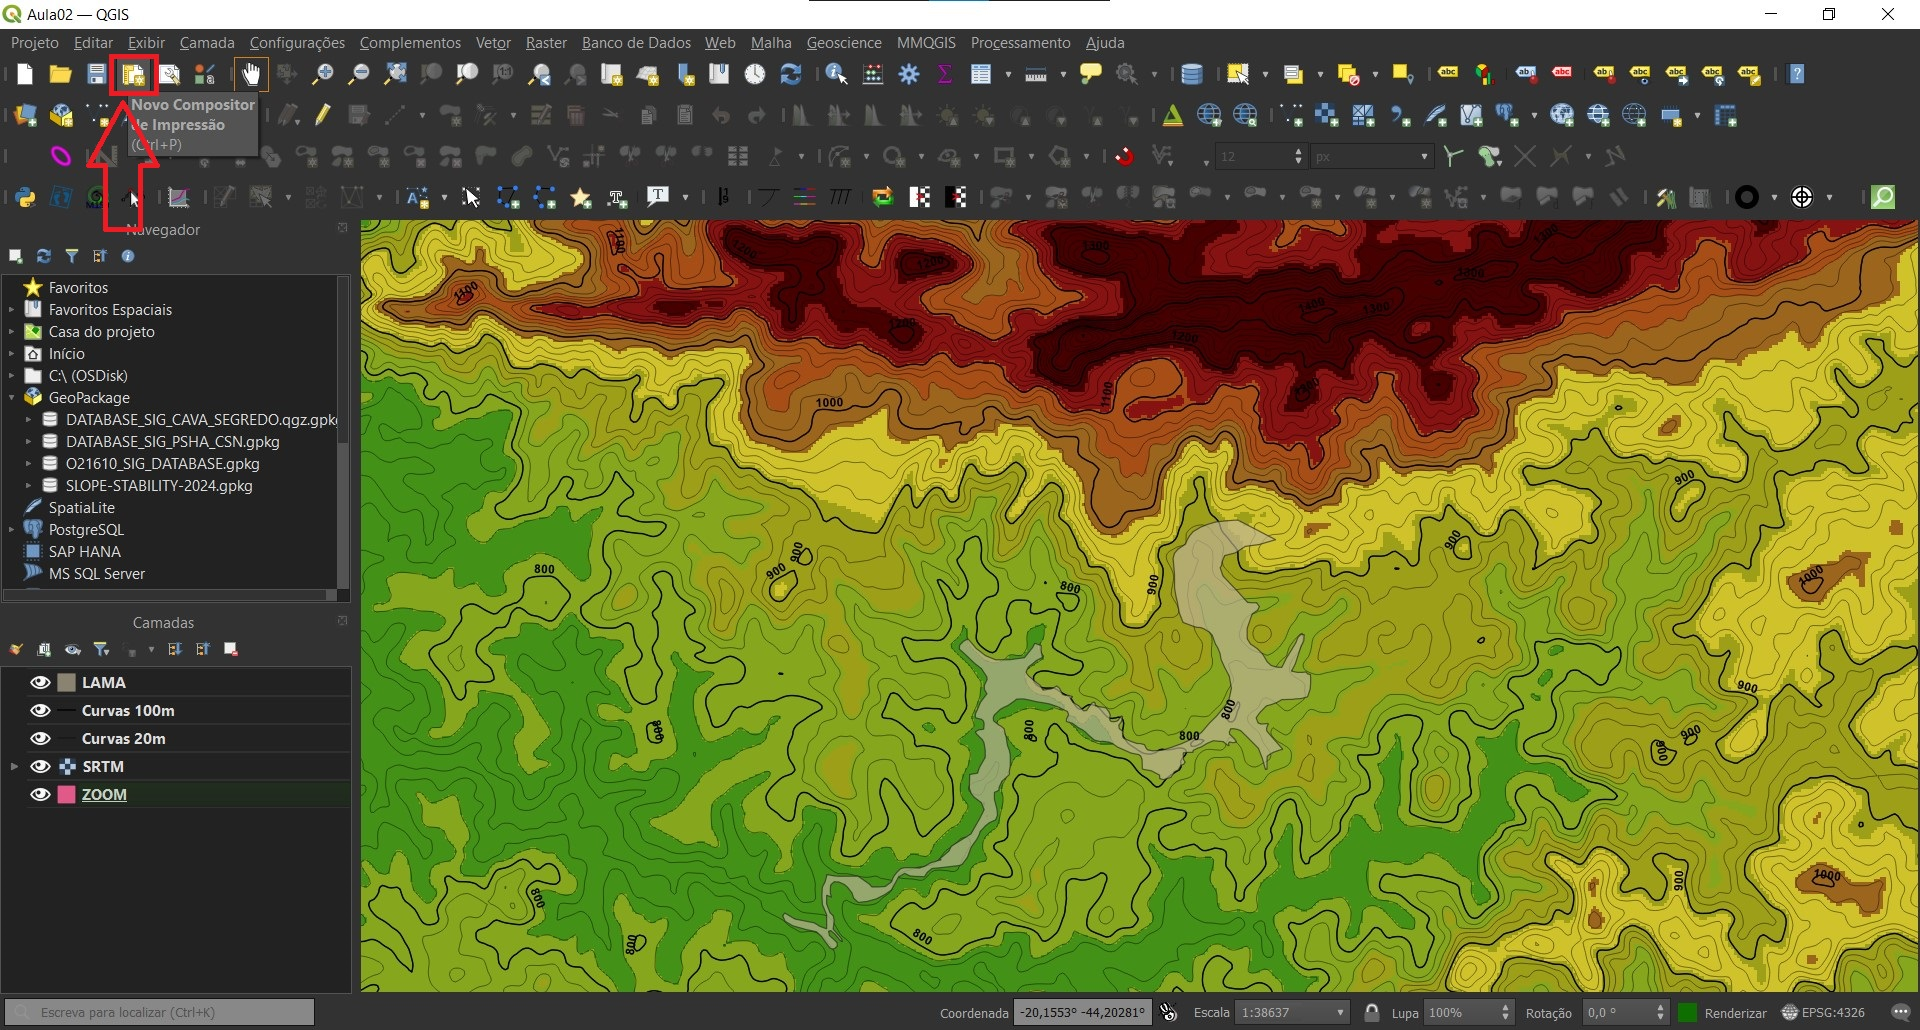
\includegraphics[width=\textwidth]{./image/comp_1}
	\end{figure}
\end{frame}

\begin{frame}
	\frametitle{Compositor de impressão}
	\begin{figure}[H]
		\centering
		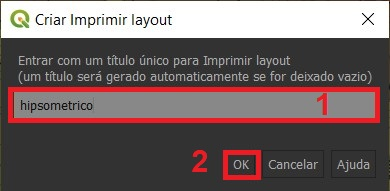
\includegraphics[width=0.7\textwidth]{./image/comp_2}
	\end{figure}
\end{frame}


\begin{frame}
	\frametitle{Compositor de impressão}
	\begin{figure}[H]
		\centering
		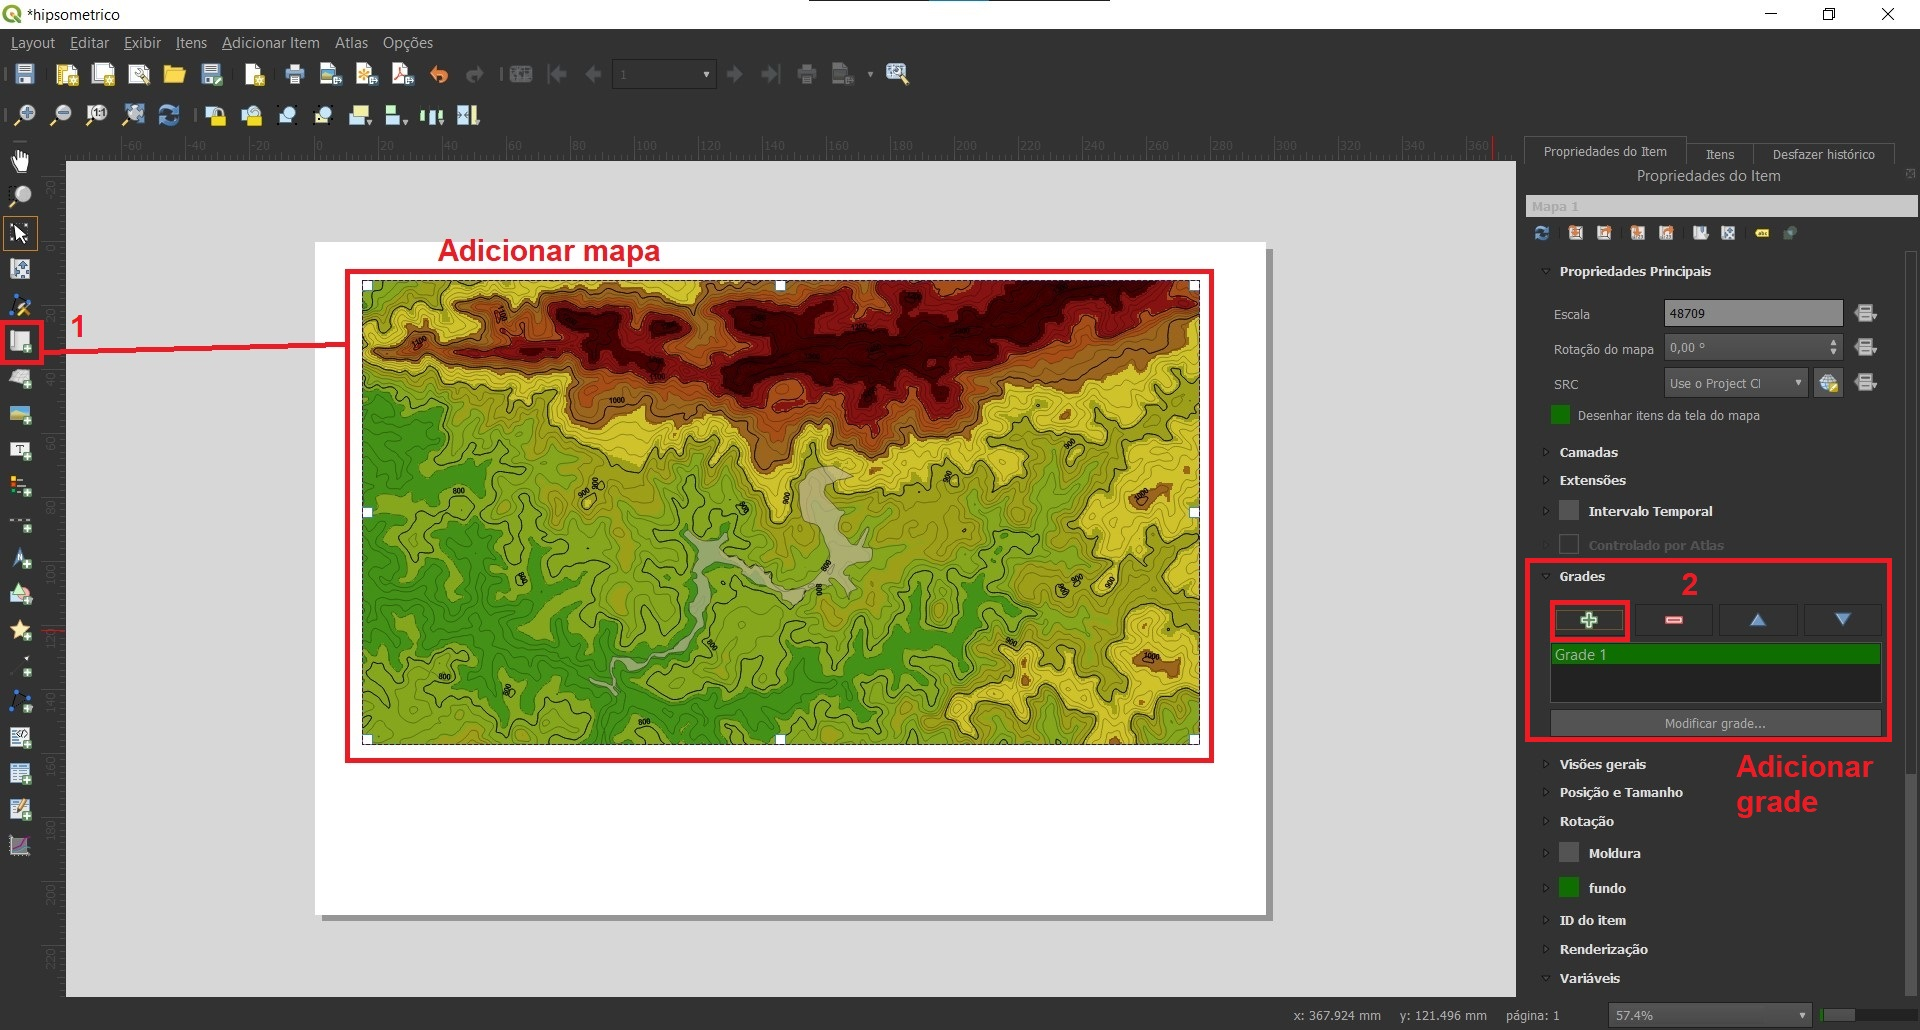
\includegraphics[width=\textwidth]{./image/comp_3}
	\end{figure}
\end{frame}

\begin{frame}
	\frametitle{Compositor de impressão}
	\begin{figure}[H]
		\centering
		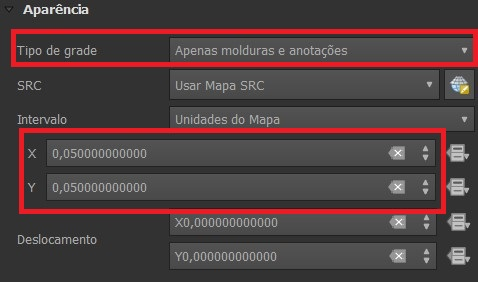
\includegraphics[width=0.49\textwidth]{./image/comp_4}
		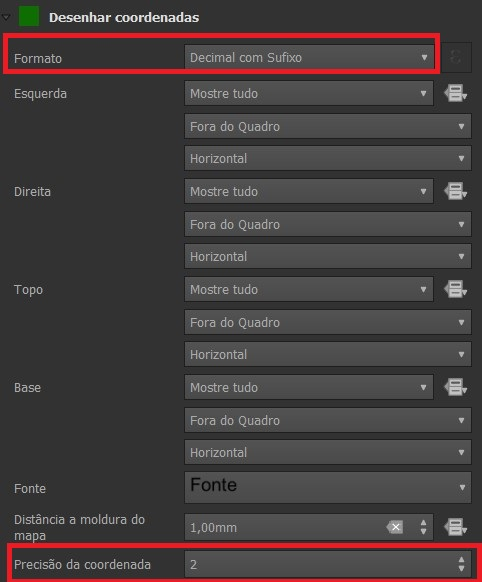
\includegraphics[width=0.49\textwidth]{./image/comp_5}
	\end{figure}
\end{frame}

\begin{frame}
	\frametitle{Compositor de impressão}
	\begin{figure}[H]
		\centering
		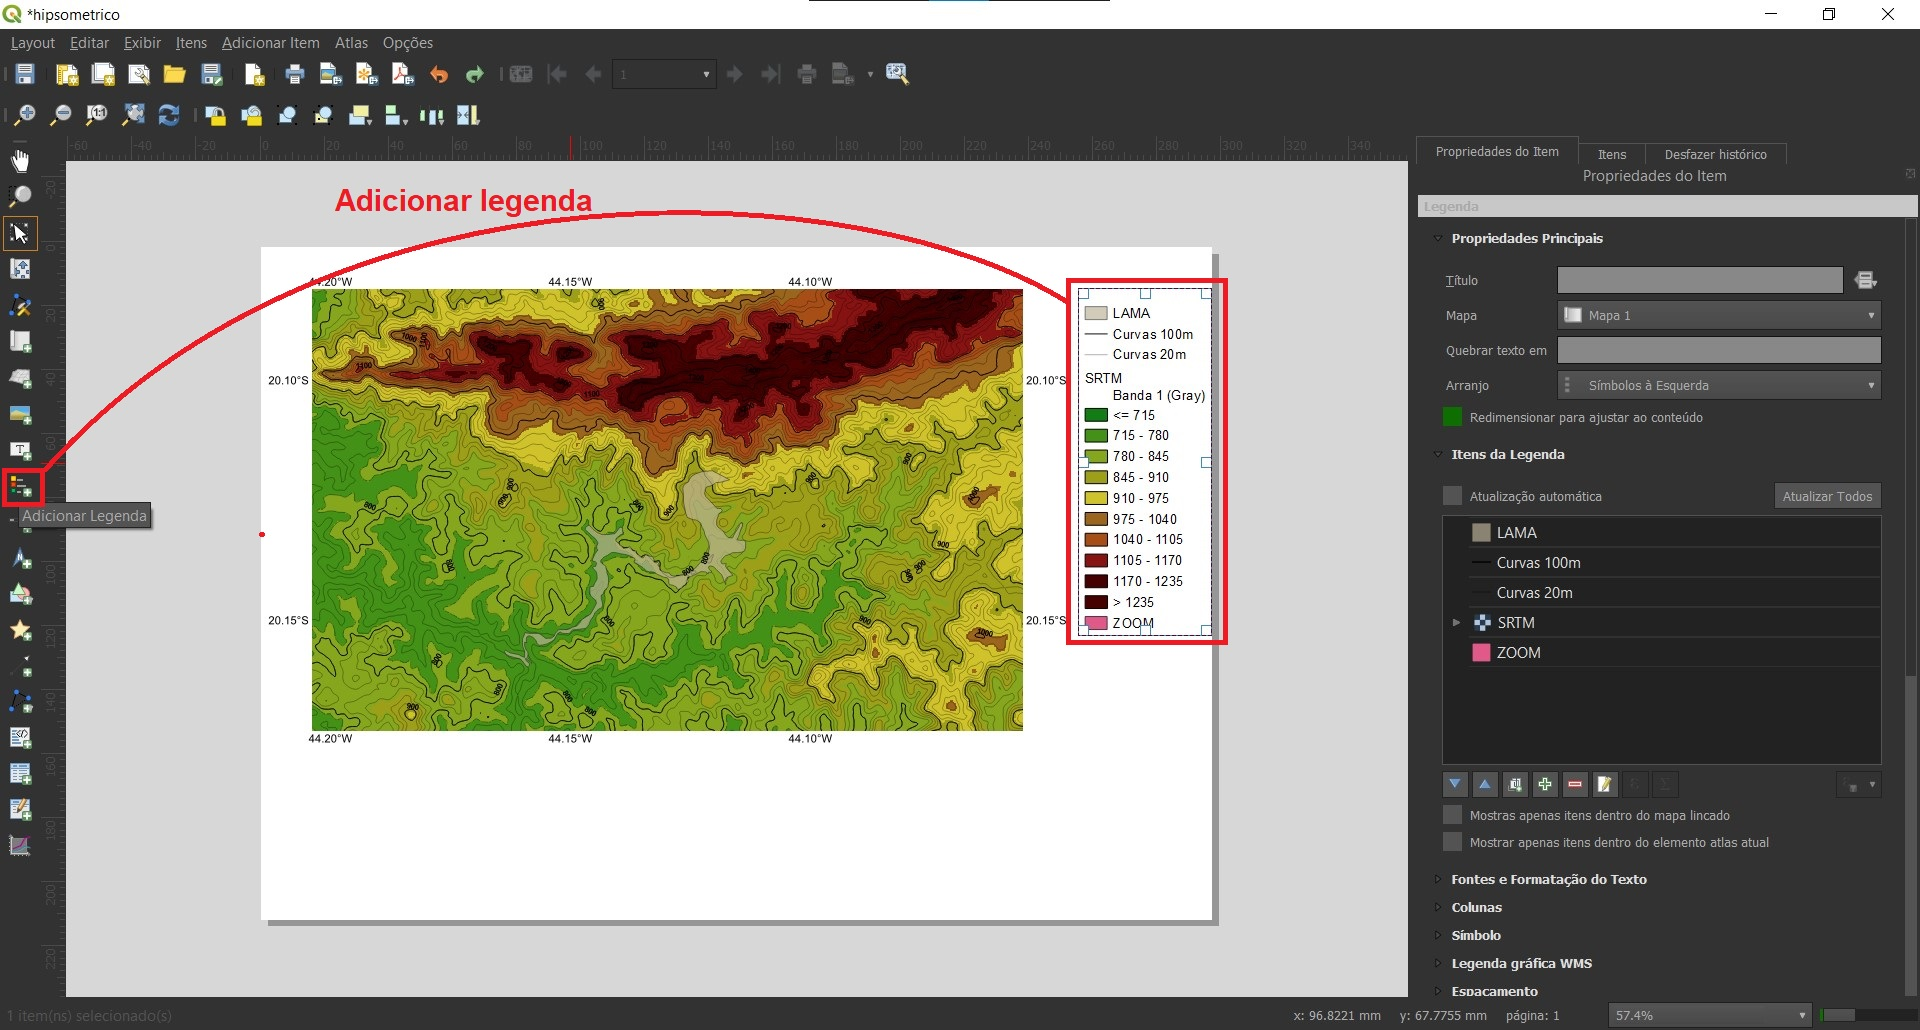
\includegraphics[width=\textwidth]{./image/comp_6}
	\end{figure}
\end{frame}

\begin{frame}
	\frametitle{Compositor de impressão}
	\begin{figure}[H]
		\centering
		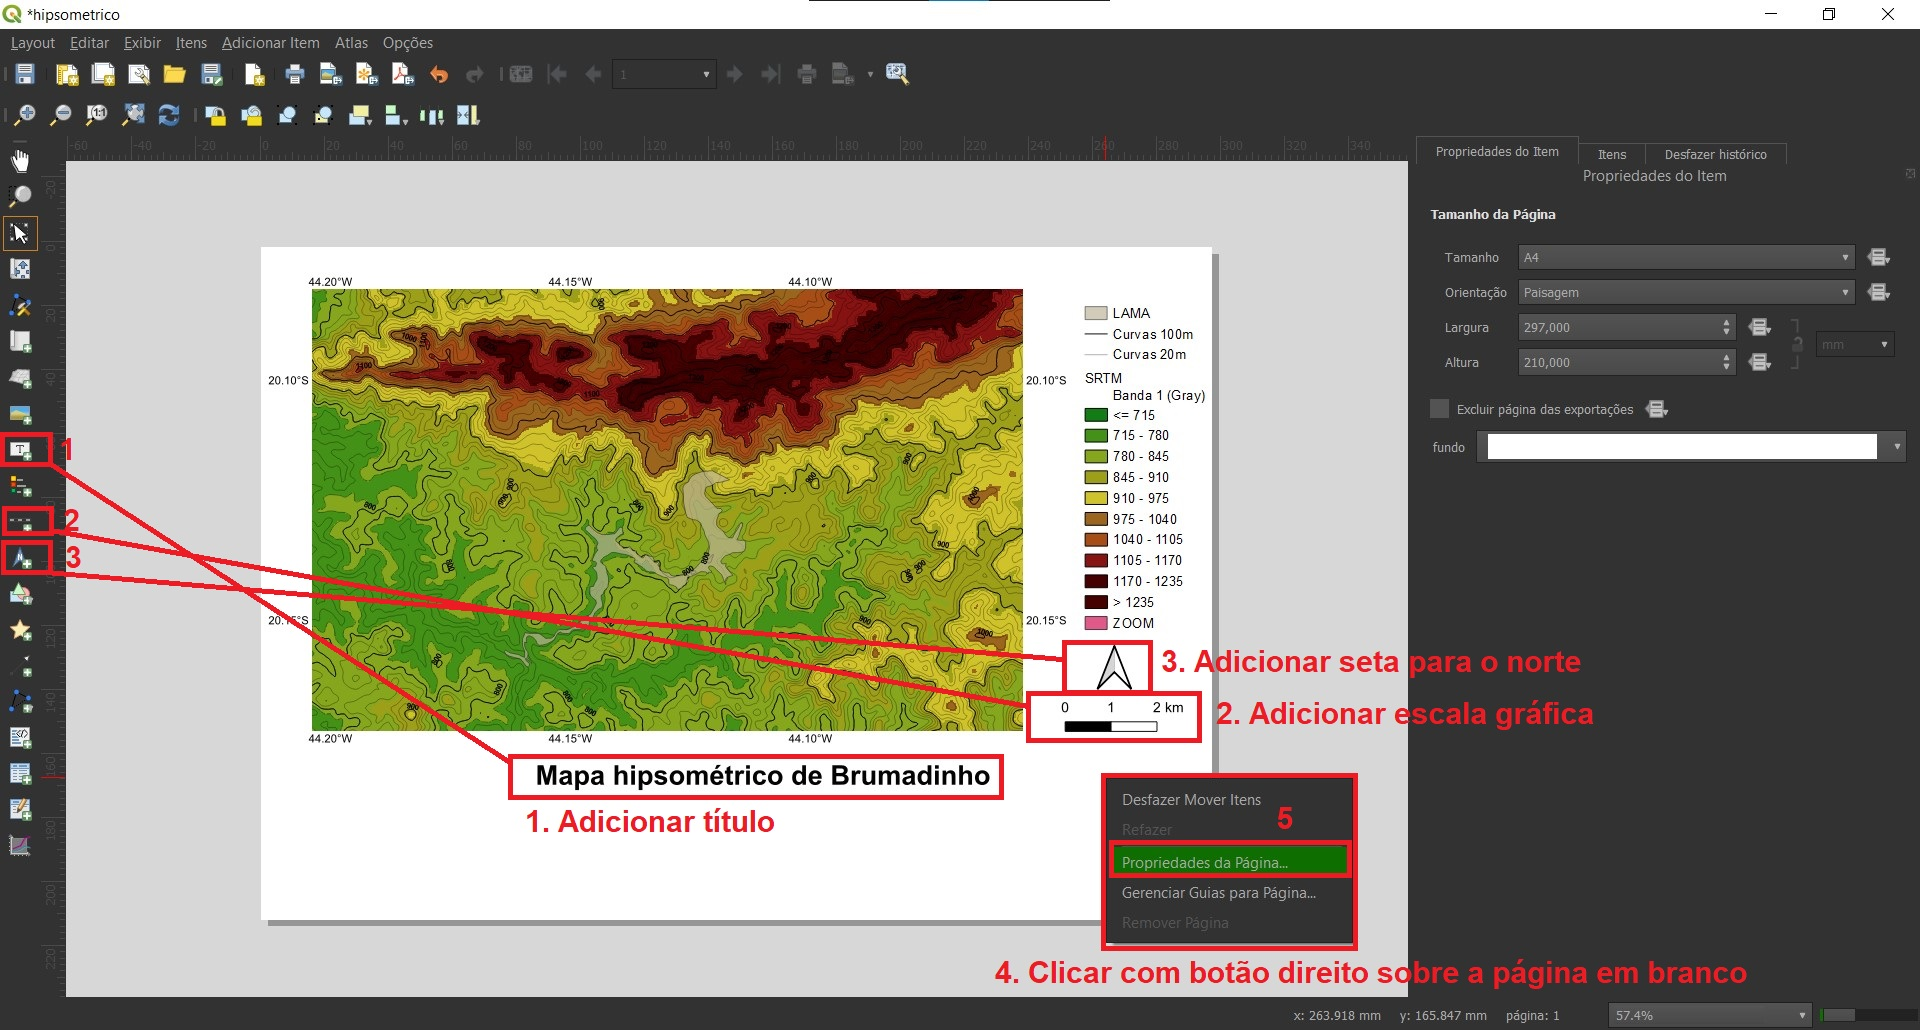
\includegraphics[width=\textwidth]{./image/comp_7}
	\end{figure}
\end{frame}

\begin{frame}
	\frametitle{Compositor de impressão}
	\begin{figure}[H]
		\centering
		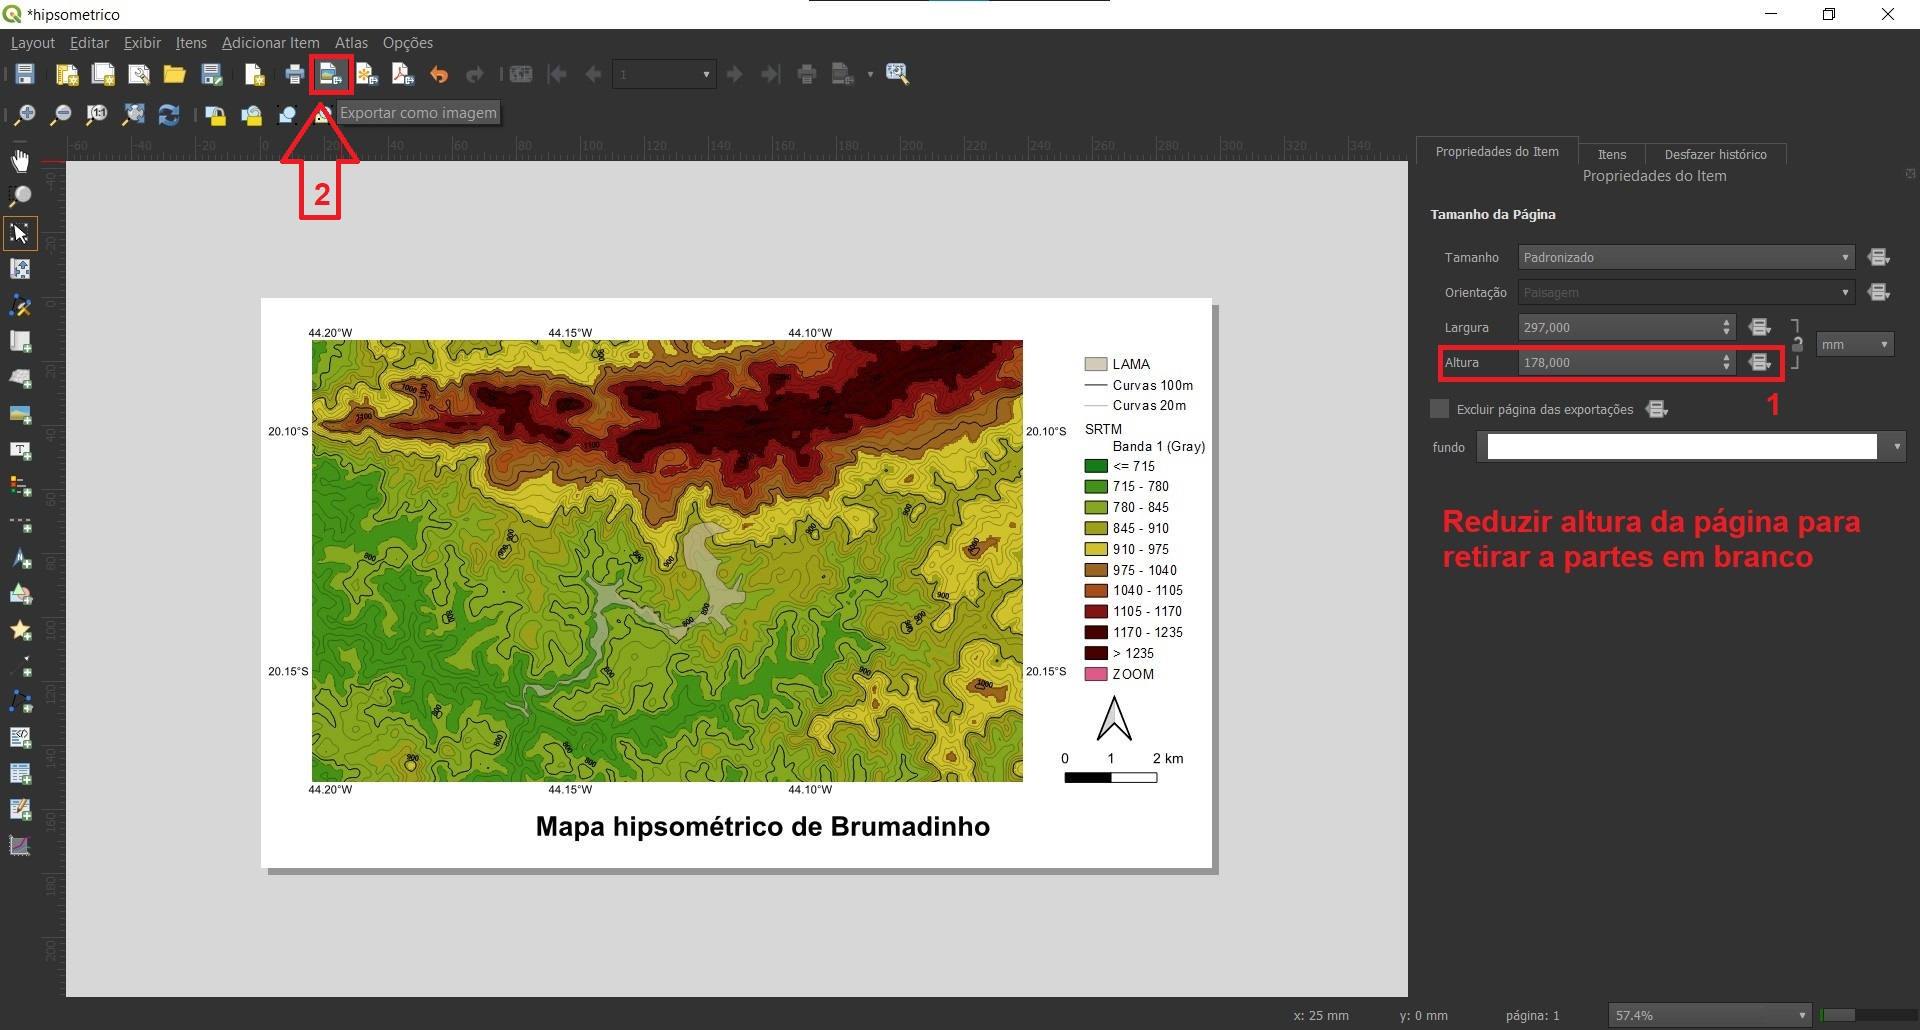
\includegraphics[width=\textwidth]{./image/comp_8}
	\end{figure}
\end{frame}

\begin{frame}
	\frametitle{Compositor de impressão}
	\begin{figure}[H]
		\centering
		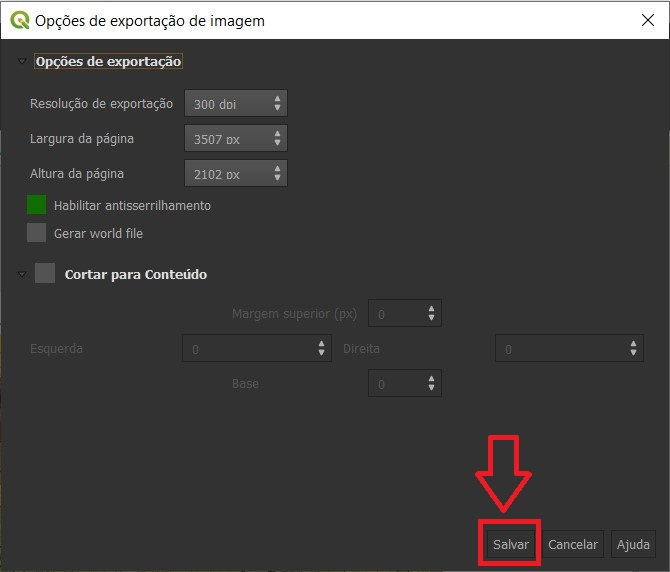
\includegraphics[width=0.7\textwidth]{./image/comp_9}
	\end{figure}
\end{frame}


%\bibliographystyle{plain}   % Alterar o estilo da referência caso necessário
%\tiny
\nocite{camara1996geoprocessamento,camara2001introduccao,fitz2008cartografia,silva2003sistemas,thiede2014quantum,tosto2014geotecnologias}
\bibliography{REF}  


\end{document}